 %================================================================================
% Erstellt am: 28.07.12
% Autor:	 Timo Amling
% Dieses Dokument beeinhaltet die gesamte Dokumentation ueber Wordpress-Pluginent-
% wicklung im Rahmen des WI-Projektes von Anatol Tissen und Timo Amling.
% Es dient primär dem Selbststudium und ist unter der GPLv3 veröffentlicht worden.
%=================================================================================

\documentclass[a4paper]{scrartcl}

%Einbinden des Headers
\usepackage[T1]{fontenc}
\usepackage[ngerman]{babel}
\usepackage{amsmath}
\usepackage[utf8]{inputenc}
\usepackage{color}
\usepackage{multirow}
\usepackage{lmodern}
\usepackage{paralist} 
\usepackage[automark]{scrpage2}
\usepackage{graphicx}
\usepackage{tabularx}
\usepackage[left]{eurosym}

%################
%--------------------------------------------------------
%pdflatex beispiel07.tex
%bibtex beispiel07
%pdflatex beispiel07.tex
%pdflatex beispiel07.tex
%pdflatex beispiel07.tex

%
\usepackage{jurabib}
%
\jurabibsetup{
	citefull=first,
	see,
	titleformat={colonsep,all},
}
\jurabibsetup{
	authorformat=year,
	commabeforerest,
	ibidem=strict,
	citefull=first,
	see,
	titleformat=colonsep,
}
\renewcommand*{\jbauthorfont}{\textsc}
%
%%Im Literaturverzeichnis werden die Titel Fett geschrieben
\renewcommand*{\biblnfont}{\scshape\textbf}
\renewcommand*{\bibfnfont}{\normalfont\textbf}
%
%%Nach den Autoren wird die Jahreszahl ausgegeben.
\renewcommand*{\jbcitationyearformat}[1]{(#1):}
\renewcommand{\jbcitationyearformat}[1]{#1:}
\renewcommand{\bibatsep}{,}
%%########################

\usepackage{multibib}
\newcites{gedr}{Gedruckte Quellen}
\newcites{int}{Internetquellen}


\usepackage[colorlinks,linkcolor=black,citecolor=black,filecolor=black,pagecolor=black,urlcolor=black,bookmarks=true,bookmarksopen=true,bookmarksopenlevel=3,plainpages=false,pdfpagelabels=true]{hyperref}

\usepackage{breakurl}

\addtokomafont{sectioning}{\rmfamily} %%Ersetzt Serif-Text durch Seriflose, nur Serif in ?berschriften
%%\***********************
%%\Kompletter Header für alle Seiten
\pagestyle{scrheadings}
%%Ersetzt Serif-Text durch Seriflose, nur Serif in ?berschriften
\renewcommand*{\headfont}{\normalfont}

%Lienienstärke für Header und Footlinie
\setheadsepline{1pt}
\setfootsepline{1pt}
%%\***********************





%%Fuer Definitionen
\usepackage{amsthm}
\newtheorem{mydef}{Definition}

%%Weitere Farben
\usepackage[usenames,dvipsnames]{xcolor}

%%Quellcode verwenden
\usepackage{listings}
\lstset{
   basicstyle=\small,
   breaklines=true,              
   keywordstyle=\color{PineGreen},
   stringstyle=\color{blue},
   commentstyle=\color{purple},
   tabsize=2,
   numbers=left,
   numberstyle=\tiny,
   numberblanklines=true,
   stepnumber=1,
   numbersep=10pt,
   xleftmargin=15pt,
   captionpos=b
 }
 \usepackage{listing}


\usepackage{setspace}
%Zeilenabstand 1,5 fach
\onehalfspacing

%Paket zur Indexerstellung
\usepackage{makeidx} 
\makeindex

%Richtige Abstände setzen
\usepackage[left=3cm,right=2cm,top=1.5cm,bottom=1cm,
textheight=245mm,textwidth=160mm,includeheadfoot,headsep=1cm,
footskip=1cm]{geometry} 


 

%Abkuerungsverzeichnis
\usepackage[
acronym,      %ein Abkürzungsverzeichnis erstellen
nonumberlist] %keine Seitenzahlen anzeigen
{glossaries}
%Den Punkt am Ende jeder Beschreibung deaktivieren
\renewcommand*{\glspostdescription}{}


\makeglossaries

\newglossaryentry{GPL}{name={GPL},
description={General Public Licence}}
\newglossaryentry{CMS}{name={CMS},
description={Content Management System}}
\newglossaryentry{API}{name={API},
description={Application Programming Interface}}
\newglossaryentry{PHP}{name={PHP},
description={PHP: Hypertext Preprocessor}}
\newglossaryentry{HTML}{name={HTML},
description={HyperText Markup Language}}
\newglossaryentry{SQL}{name={SQL},
description={Structured Query Language}}
\newglossaryentry{XAMPP}{name={XAMPP},description={Cross-plattform, Apache, MySQL, PHP, Perl}}
\newglossaryentry{URL}{name={URL},description={Uniform Resource Locator}}
\newglossaryentry{CSS}{name={CSS},description={Cascading Style Sheets}}
\newglossaryentry{FTP}{name={FTP},description={File Transfer Protocol}}
\newglossaryentry{POT}{name={POT},
description={Portable Object Template}}
\newglossaryentry{ID}{name={ID},
description={Identifier}}
\newglossaryentry{URI}{name={URI},
description={Uniform Ressource Identifier}}
%##### ANFANG DOKUMENT #### 
\begin{document}

%Einbinden der Titels
\begin{titlepage}

\includegraphics[scale=1.0]{pictures/logoheader.jpg}\\
\begin{center}
\Large
Fachhochschule Köln\\
Fakultät für Informatik und Ingenieurwissenschaften
\hrule\par\rule{0pt}{2cm} 
\LARGE
\textsc{W I - P r o j e k t}\\
\vspace{1cm}
\huge
{\bf Wordpress Plugin-Entwicklung}\\
\Large
Die Entwicklung eines Plugins zur Mentorensuche für das Programm {\it Mentoring4Excellence}\\
\vspace{1.0cm}
\large
{\bf Vorgelegt an der} \\
Fachhochschule Köln, \\
Campus Gummersbach\\
im Studiengang\\
Wirtschaftsinformatik\\
\vspace{1.0cm}
\textbf{Ausgearbeitet von:}\\
\textsc{Amling, Timo - 1107\\
Tissen, Anatol - 1107\\}
\vspace{2.0cm}
\begin{tabular}{ll}
 \textbf{Projektbetreuung:} & Frau Prof. Dr. Heide Faeskorn-Woyke \\
 \textbf{Fachbetreuung:} & Herr B.Sc. Ludger Schönfeld\\
 \end{tabular}
 \vspace{1.5cm}
 \\Gummersbach, im März 2013
\end{center}

\end{titlepage}

%Einbinden des Inhaltsverzeichnis
%Diese Seite wird nicht mitgezählt
\thispagestyle{empty}

%Inhaltsverzeichnis erzeugen
\tableofcontents \label{inhaltsverzeichnis}

%Diese Seite wird nicht mitgezählt
%InhVer geht ueber 2 Seiten, deswegen hier nochmal
\thispagestyle{empty}

%%\Tiefe des zu gliedernden Inhaltes festlegen
\setcounter{tocdepth}{4}   
\setcounter{secnumdepth}{4}   

\newpage

%Einbinden von Abbildungs-, Abkürzungsverzeichnis
%Abbildungsverzeichnis erzeugen
\thispagestyle{empty}
\listoffigures

%Zwischen den Verzeichnissen eine neue Seite einbinden
\newpage

%Tabellenverzeichnis erzeugen
\thispagestyle{empty}
\listoftables

%Zwischen den Verzeichnissen eine neue Seite einbinden
\newpage

%%Glossar (Abkuerzungsverzeichnis einbinden)
\thispagestyle{empty}
\printglossary[title=Abkürzungsverzeichnis]
%Zwischen den Verzeichnissen eine neue Seite einbinden
\newpage

%Quellcodeverzeichnis erzeugen
\thispagestyle{empty}
\renewcommand\lstlistlistingname{Quellcodeverzeichnis} 
\lstlistoflistings 





\thispagestyle{empty}
%Zähler für Kapitel auf 1 setzen
\setcounter{page}{0}

\newpage

%%%********************************************************************************
\section{Einleitung}\label{sec_Einleitung}
Dieses Tutorial soll anhand von Erklärungen und Beispielen eine Übersicht über die Pluginentwicklung für ein Wordpresssystem geben. \newline
Dabei wird anhand von verschiedener Fachliteratur auf einzelne Themengebiete eingegangen und diese dann im Detail behandelt. \newline
Die zentrale Fragestellung lautet dabei: Wie entwickel ich ein Plugin in Wordpress. Dabei wird  sich am Beispiel an dem Projekt "mentoren-suche", welches für das Programm \emph{Mentoring4Excellence} programmiert wurde, orientiert.
\subsection{Zielsetzung}
Ziel dieser Arbeit ist dem Leser eine Übersicht über die Techniken, die für die Pluginentwicklung benötigt werden, zu geben.\newline
Dabei lässt sich aufgrund der beschränkten Zeit nicht auf jedes Detail genauestens eingehen. Kenntnisse in den Programmiersprachen PHP, HTML und CSS sind Voraussetzung, um die einzelnen Anweisungen zu verstehen. 
\subsection{Motivation}
Das Tutorial wurde im Rahmen des WI-Projektes von den beiden Studenten Timo Amling und Anatol Tissen geschrieben, welche zuvor auch das dazugehörige Plugin entwickelt und dokumentiert haben.\newline
Daher haben die Autoren die ersten Praxiserfahrungen mit dem Umgang professioneller Pluginentwicklung kennengelernt und möchten mit diesem Tutorial ihre Erfahrungen und Wissen einem breiteren Spektrum an Informatiker, Studenten und Informatikinteressierte weitergeben.\newline
Anbei soll an dieser Stelle auch erwähnt werden, dass das Kapitel \ref{interundlok} von Herrn Ludger Schönfeld geschrieben wurde. Wir danken ihn an dieser Stelle vorab für seine konstruktive Mitarbeit.
\subsection{Inhalt}
In diesem Unterkapitel wird neben einer Übersicht über die einzelnen Kapitelinhalte auch der Aufbau dieses Tutorials begründet. 
\subsubsection{Kapitelübersicht}
Nachdem in diesem ersten Kapitel \nameref{sec_Einleitung} unter anderem die Motivation dieses Tutorials geklärt wurde, wird im  zweiten Kapitel \nameref{Vorbereitung} eine Übersicht über Wordpress behandelt. Dabei wird sich mit dem Begriff des Plugins, sowie die benötigten Entwicklungswerkzeuge und Standards für die Programmierung eingegangen.\newline
Anschließend wird in Kapitel \nameref{AUFBAUPLUGIN} die grundsätzliche Struktur eines jeden Plugins, was Funktionen sind und wie diese geschrieben werden, beschrieben.\newline
Danach kommt das 4te Kapitel, \nameref{shortcodes}. Dieses Kapitel widmet sich den kleinen Codeschnipseln, welche an beliebiger Stelle im Seiteninhalt eingebaut werden können. Dabei wird sich auch der Shortcode-API angesprochen.\newline
Im Kapitel \nameref{DBzugriff} werden alle technischen Aspekte, die benötigt werden um mit einer Datenbank über ein Plugin zu kommunizieren beschrieben.\newline
Anschließend wird im Kapitel \nameref{PLASDA} die zwei wesentlichen Aspekte eines Plugins aus Anwendersicht besprochen: Die Installation und Deinstallation eines Plugins.\newline
In Kapitel \ref{Formular} wird sich zunächst dem Begriff des Formulars gewidmet, anschließend wird beschrieben, wie Formulare erstellt und verwendet werden.\newline
Nachdem die rudimentären technischen Aspekte in den vorherigen Kapiteln erläutert wurden, widmet sich das Kapitel \nameref{interundlok} der Sprachanpassung für Plugins. Nach einigen Begrifflichkeiten, wird anschließend gezeigt, wie Übersetzungen erstellt und auf den neusten Stand gehalten werden. Natürlich spielt auch das laden einer solchen Textdomain in diesem Kapitel eine Rolle.\newline
Das letzte Kapitel \nameref{fazit} beschreibt zusammenfassend die einzelnen oben genannten Schritte der Pluginentwicklung. 
\subsubsection{Aufbau}
In diesem kleinen Abschnitt geht es um die grundsätzliche Frage nach dem strukturellen Aufbau dieses Tutorials. \newline
Wie sich erkennen lässt, behandeln die ersten drei Kapitel inhaltlich die ersten Schritte in der Plugin-Entwicklung.  Dabei wird immer spezifischer von der Klärung des Begriffs \emph{Plugin} über entsprechende Werkzeuge und Normen bis zur Aktivierung und den ersten Schritten zum eigenen Plugin beschrieben. \newline
Die Kapitel vier bis acht dienen der tieferen und komplexeren Entwicklung. Dort werden spezielle Techniken angesprochen. Angefangen mit dem verwenden von Shortcodes um das Plugin auf eine Wordpress-Seite einzubinden, wird anschließend Aspekte der Datenbankkommunkation besprochen. Auch Sicherheitsaspekte was beispielsweise bestimmte Angriffstechniken auf die Datenbank angehen, werden hier beachtet. \newline
Weiter geht es dann mit Formularen in Kapitel sieben. Neben einigen grundsätzlichen Methoden und Begriffen, wird anschließend gezeigt, wie Formulare in Wordpress erstellt werden. Dies wird dann zum Abschluss des Kapitels mit Beispielen aus der Mentoren-Suche abgerundet.\newline
Im achten Kapitel - der Internationalisierung und Lokalisation - geht es um die Sprachanpassung eines Wordpress-Plugins. Dabei werden nach einer kurzen Einführung in das Thema einige Techniken gezeigt, sich Übersetzungen erstellen lassen und diese im einzelnen konfiguriert werden. wie.\newline
Im neunten Kapitel werden dann die Installation und Deinstallation aus Anwendersicht beschrieben, um das Tutorial abzuschließen und aus der Entwicklersicht wieder auf die Anwendersicht zu kommen. \newline
Zum Schluss werden dann im Kapitel neun die wichtigsten Fakten aufgelistet und dient so als Rückblick auf den Inhalt. Weiterhin wird auch hier ein Ausblick gegeben. Dies rundet dann das Tutorium sinnvoll ab.
\newpage
%
%%%********************************************************************************
\section{Vorbereitung}\label{Vorbereitung}
In diesem Kapitel werden grundlegende Begriffe für den Umgang mit einem \gls{CMS} wie Wordpress erklärt und erläutert. Darauf aufbauend wird in die Definition eines Plugins gegangen. Zum Abschluss werden anschließend die wichtigsten Werkzeuge zur Pluginentwicklung vorgestellt.
\subsection{Was ist Wordpress?}
Laut Bondari und Griffiths\footcitetgedr[Vgl.][Seite 7]{BB11} lässt sich Wordpress als \gls{CMS} beschreiben, welches hauptsächlich für Blogs genutzt wird. Dieses Projekt besteht seit 2003 und hat sich seitdem als eines der weit verbreiteten Blogging-Software entwickelt. \newline
Als \gls{CMS} lässt sich ein System beschreiben, mit welchem sich Daten auf einer Website dynamisch verwalten lassen. Drei wichtige Punkte sind hierbei zu beachten, um von einem vollwertigen \gls{CMS} zu sprechen. Dies ist zum einem die Tatsache, dass Benutzer nicht tief in die Programmierung eingreifen müssen, um die Website im Aufbau zu verändern.\footcitet[Vgl.][Seite 24]{AH12}\newline
Im Wikipedia-Eintrag für Wordpress\footcitetint[Vgl.][]{WIKWP12} finden sich die anderen beiden Punkte. Diese lauten zum einem, dass Benutzerrollen und deren Rechte verwaltet werden können. Es gibt also eine Möglichkeit, verschiedenen Benutzer, unterschiedliche Rechte zuzuteilen. Gleichzeitig ist es aber auch möglich, dass mehrere Benutzer gleichzeitig Inhalte bearbeiten und anpassen können.\newline
Der letzte Punkt handelt von der Erweiterbarkeit eines \gls{CMS}, nämlich die Möglichkeit, externe Plugins in das System einzubinden. All die aufgezählten Punkte werden von Wordpress erfüllt, sodass sich von einem  vollwertigen CMS sprechen lässt. \newline
Die Software ist laut wordpress.org\footcitetint[Vgl.][]{GNU312} unter der \gls{GPL} lizensiert. Dies bedeutet, dass Wordpress frei von jedem verwendet werden darf, sei es im privaten oder kommerziellen Bereich. Dabei wird die Software und der Quellcode kostenfrei zur Verfügung gestellt und kann von jedem verwendet und weiterentwickelt werden.\newline
Von Hause aus bietet Wordpress nur eine begrenzte Funktionalitäten, welche jedoch mit Plugins erweiterbar sind. Diese werden oft von engagierten Programmierern aus der Wordpressgemeinschaft programmiert, um wünschenswerte Funktionalitäten einzubauen und so die Software zu erweitern.\footcitetgedr[Vgl.][Seite 22]{AH12}
\subsection{Was ist ein Plugin?}\label{WIEP}
Plugins sind Erweiterungen für Wordpress. Sie dienen dazu, das System mit bestimmten Funktionalitäten zu erweitern und liegen im Plugin-Verzeichnis \emph{/wp-content/plugins/}. Wordpress unterscheidet  nicht wie andere CMS in bestimmte Module oder Addons. Für Wordpress ist jeder Quellcode, der das System erweitert ein Plugin.\newline
Um diese Plugins zu programmieren, bietet Wordpress eine eigene Schnittstelle für Programmierer an: das sogenannte \gls{API}.
Hiermit können Programmierer mit dem System über bestimmte Funktionen und Variablen kommunizieren. Der größte Teil der Funktionen ist prozedural in \gls{PHP}, \gls{HTML} und teils in \gls{CSS} geschrieben.  
Da es sich um sehr viele Funktionen handelt, muss bei der eigenen Programmierung darauf geachtet werden, dass Namen für Funktionen nicht doppelt vorkommen. Dies könnte zu Namenskollisionen mit anderen Funktionen führen. Diese Thematik wird tiefer im Unterkapitel \nameref{PRST} behandelt.\newline
Zum Schluss dieser Einführung wird noch der Begriff \emph{eventorientiert} erklärt und erläutert. Dies ist die Architektur, nach der Plugins in Wordpress arbeiten\footcitetgedr[Vgl.][Seite 9 - 10]{BB11}.\newline
Kurz gesagt bedeutet dieser Begriff, dass über sogenannte \emph{hooks}, Kontakt zur Wordpress-Schnittstelle aufgebaut werden kann. Dabei wird in einem bestimmten Bereich der Seite entweder eine neue Funktion eingebaut (dann ist es ein \emph{action\_hook}) oder bestimmter Inhalt gefiltert (dann ist es ein \emph{filter\_hook}).\footcitetgedr[Vgl.][Seite 274]{AH12}\newline
Hooks sind also ein Platz auf einer Seite, an der sich frei übersetzt Quellcode ''aufhängen'' lässt. Die eventorientierte Architektur bietet also die Möglichkeit, erst bei einem Klick auf ein bestimmtes Objekt, einen hook auszulösen. In HTML wäre ein hook die Funktion hinter dem Button ''Button anklicken''\footcitetgedr[Vgl.][Seite 10]{BB11}. Tiefer wird auf die eventorientierte Architektur im Kapitel \ref{benutzerdeffunkt} eingegangen.\newline
Soviel zu dem Begriff des Plugins. Im \ref{BEWE} geht es nun um die Entwicklungsvorbereitung. Dabei werden verschiedene Umgebungen und Programme vorgestellt. 
\subsection{Benötigte Werkzeuge}\label{BEWE}
Hier werden nun die Werkzeuge vorgestellt, welche für die Entwicklung und dem eigentlichen Umgang mit Wordpress benötigt werden. Hierzu wird auf der einen Seite Wordpress, aber natürlich auch eine Umgebung für die Programmierung, zum Testen und Hochladen benötigt.
\subsubsection{Webserver}
Der Webserver muss laut offiziellen Vorgaben\footcitetgedr[Vgl.][Seite 11]{BB11} von Wordpress mindestens \gls{PHP} 5.2 und MySQL 4.1.2 \gls{SQL} für die von uns verwendete Wordpressversion 3.2 unterstützen. \newline
Wir haben dafür eine lokale Installation mittels \gls{XAMPP} verwendet. \gls{XAMPP} kann unter \url{http://www.apachefriends.org/en/xampp.html} heruntergeladen werden.
\subsubsection{Wordpress}
Wordpress bietet unter \url{http://wordpress.org/download} die aktuellste Version seines Softwarepakets an. Dieses ist gepackt und muss anschließend nur noch auf den Webserver im \emph{htdocs}-Ordner entpackt werden. Anschließend wird  die \gls{URL} \url{http://localhost/wordpress/} oder \url{http://deine-domain/wordpress/} aufgerufen und die entsprechenden Datenbank-Details eingeben werden.\footcitetgedr[Vgl.][Seite 48]{AH12} \newline
Da die Pluginprogrammierung hier im Mittelpunkt steht, wird nicht weiter auf dieses Thema eingegangen. Für unser Plugin ist es erforderlich  eine Version über 3.0 zu nehmen, da es ansonsten zu Fehlern kommen kann.
\subsubsection{Editor}
Als Editor zum programmieren der einzelnen Funktionen ist kein spezieller erforderlich. Allerdings sollte darauf geachtet werden, dass dieser entsprechende Anforderungen entspricht\footcitetgedr[Vgl.][Seite 12-13]{BB11}:
\begin{enumerate}
	\item Syntax-Highlighting
	\item Anzeige von Zeilennummern
	\item Anzeige von zusammengehörigen Klammern
\end{enumerate}
Bei der Mentoren-Suche wurde für Windows das Programm Notepad++ verwendet, welches sich unter \url{http://notepad-plus-plus.org/download} herunterladen lässt und frei verfügbar ist. \newline
Für Mac-Systeme kann das Programm \emph{textwrangler} verwendet werden.. Dies ist ein proprietäres Programm, welches kostenlos unter folgenden Link \url{http://www.barebones.com/products/TextWrangler/} heruntergeladen werden kann.
\subsubsection{FTP Client}
Um vom lokalen Rechner Dateien auf den Server zu transportieren, wird ein \gls{FTP}-Client benötigt. Dafür kann unter Windows das Programm Filezilla verwendet werden. Es handelt sich hierbei um ein unter der \gls{GPL} lizenzierten Programm. \newline
Für Mac OS X kann das Programm Cyberduck verwendet werden. Auch hierbei handelt es sich um \gls{GPL}-lizenziertes Programm.\footcitetgedr[Vgl.][Seite 14]{BB11}
\subsection{Programmierstandards}\label{PRST}
Standards für Programmierer sind deshalb sehr wichtig, weil damit auch andere Programmierer den logischen Aufbau des Plugins schnell verstehen können - auch wenn diese manchmal nicht mit den eigenen Ideen zufrieden sind. Die Hauptpunkt, um den eigenen Quellcode möglichst gut zu organisieren und strukturieren, werden an dieser Stelle nach Bondari und Griffiths\footcitetgedr[Vgl.][Seite 15 - 18]{BB11} aufgezählt:
\begin{enumerate}
	\item {\bf Aufgaben werden in Prozeduren eingeteilt}
	\begin{itemize}
	 \item Für jede Aufgabe gibt es genau eine Prozedur, welche aber auch andere Prozeduren aufrufen kann. Eine Regel hierbei ist, dass nicht mehr als drei Variablen der Prozedur übergeben werden sollen. 
	\end{itemize}
	\item {\bf Es werden Klassen verwendet}
	\begin{itemize}
		\item Je mehr programmiert wird, desto mehr wird in die objektorientierte Programmierung eingestiegen, da mit diesem Programmierparadigma Vererbung, Erweiterungen und Klassen besser programmiert werden können. Eine prozedurale Programmierung mit Klassen ist auch möglich. Wir haben uns aufgrund von nur drei Entwicklern und diesem vergleichbar kleinen Projekt für die prozedurale Programmierung entschieden.
	\end{itemize}
	\item {\bf Verwendung von beschreibenden Variablen und Funktionen}
	\begin{itemize}
		\item Für \gls{PHP} gibt es keine großen Anforderungen an eine Variable, was den Namen angeht. Allerdings sollte immer darauf geachtet werden, dass Variablen den entsprechenden Kontext, möglichst kurz und auf Englisch wiedergeben sollten. Wenn der Quelltext mit Variablen bestückt ist, die sich nicht von selbst erklären, fällt es sehr schwer die Logik des Programms zu verstehen.	
	\end{itemize}
	\item {\bf Verwendung von modularer Programmierung}
	\begin{itemize}
	\item	 Indem modulare Programmierung verwendet wird, können einzelne Klassen beispielsweise für andere Projekte verwendet werden, da diese übersichtlich abgespeichert werden.
	\end{itemize}
\end{enumerate}
In dem Projekt der Mentoren-Suche wurde versucht, sich an diese Standards zu halten. Deshalb soll in diesem Tutorial nicht davon abgewichen werden.

\newpage
%% 	
%%%%********************************************************************************
\section{Aufbau des Plugins}\label{AUFBAUPLUGIN}
In diesem Kapitel wird der grundsätzliche Aufbau eines Plugins besprochen. Dabei werden neben allgemeinen Details, wie die Aktivierung eines Plugins, auch einzelne Programmierdetails angesprochen. Inbegriffen sind hierbei der erste Abschnitt eines jeden Plugins: der \nameref{ACHE}, sowie die einzelne Funktionen und wie diese referenziert werden.
\subsection{Allgemeines}
Ein paar Details zur Programmierung von Plugins wurden bereits im Unterkapitel \ref{WIEP} angesprochen - beispielsweise eine Einleitung zu hooks.\newline
Nach Hetzel\footcitetgedr[Vgl.][Seite 274]{AH12} gibt es jedoch einige technische Details, mit welchen sich der Programmierer beschäftigen muss, bevor die eigentliche Programmierung beginnen kann. Zunächst ein Detail, welches auch in \nameref{WIEP} angesprochen wurde, jedoch von außerordentlicher Wichtigkeit ist: Plugins werden generell unter Wordpress in dem Plugin-Ordner {\emph{/wp-content/plugins/}}. Dies hat den wichtigen Grund, dass Wordpress nur Plugins erkennt, welche auch in diesem Ordner kopiert worden sind. Weiterhin bietet es sich an, für jedes Plugin einen eigenen Unterordner zu erstellen, um so die Übersichtlichkeit bei dem Einsatz mehrerer Plugins zu gewährleisten. Auch sollte die Hauptdatei des Plugins immer den Namen des Plugins haben und eine Namenskonvention, welche nicht mit anderen Plugins in Konflikt kommt, eingehalten werden.\newline
An dieser Stelle möchten wir vorstellen, wie die Details für das Plugin Mentoren-Suche aussehen:
\begin{enumerate}
	\item Als Hauptordner unter dem Pluginverzeichnis {\emph{/wp-content/plugins}} haben wir {\emph{mentoren-suche}} gewählt 
	\item Die Hauptdatei unseres Plugins lautet {\emph{mentoren-suche.php}}
\end{enumerate}
Soviel zu den Details für die Vorbereitung der Programmierung. Im nächsten Abschnitt wird erläutert, wie das Plugin aktiviert wird.
\subsection{Aktivierung des Plugins}\label{aktivierungplugin}
Insgesamt gibt es aus Anwendersicht drei Schritte\footcitetgedr[Vgl.][Seite 29]{BB11}, um ein Plugin zu aktivieren:
\begin{enumerate}
	\item Als erster Schritt wird zum Wordpress Dashboard navigiert ({\emph{http://localhost/wp-admin/} oder \emph{http://deine-domain/wp-admin/}})
	\item Anschließend wird die Option {\emph{Plugins}} ausgewählt
	\item Als letzter Schritt wird auf {\emph{Aktivieren}}	des entsprechenden Plugins ({\emph{mentoren-suche}}) geklickt
\end{enumerate}
Soviel einmal zur Theorie. Der nächste Abschnitt leitet in die Praxis der Aktivierung.
   \begin{figure}[htbp]
	\begin{center}
		
\includegraphics[angle={360}, scale=0.61]{pictures/plugin_deak.jpg}
	    \caption{Pluginübersicht im Pluginmenü}
	    \label{img:ERFMELDPM}
	    	\end{center}
   \end{figure} 
Zur besseren Übersichtlichkeit und für eine ersten Eindruck des fertigen Plugins, ist in Abbildung 
\ref{img:ERFMELDPM} das Pluginmenü mit den entsprechenden Informationen aus dem im nächsten Unterkapitel \nameref{ACHE} abgebildet.
   \begin{figure}[htbp]
	\begin{center}
	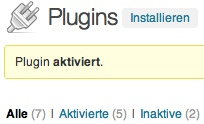
\includegraphics[angle={360}, scale=0.61]{pictures/plugin_akt.jpg}
	    \caption{Erfolgreiche Meldung der Aktivierung}
	    \label{img:ERFMELDAK}
	\end{center}
   \end{figure}\newline
Nach einem Klick auf \emph{Aktivieren} ist das Plugin aktiviert und es erscheint die in Abbilung \ref{img:ERFMELDAK} abgebildete Meldung.
Während der Aktivierung werden verschiedene Funktionen ausgeführt. Beispielsweise wird im Backend-Menü in der Menüstruktur angelegt oder es wird geprüft, ob die benutzte Wordpressversion mit dem Plugin kompatibel ist. Weiterhin steht auch nun der Shortcode für das Plugin bereit und die Übersetzungen der einzelnen Textelemente werden angezeigt. \newline
Wie dies alles zu programmieren ist, wird in dem nächsten Kapiteln besprochen. Dabei wird als erstes auf den Informationen Header, anschließend auf einzelne Funktionen und abschließend die Hooks besprochen. Soviel erst einmal zur Aktivierung und kleinen technischen Hintergrundabläufen. 
\subsection{Information Header}\label{ACHE}
In Wordpress ist der {\emph{Information Header}} in der Pluginentwicklung immer der erste Teil des Programmes. Er wird dafür benötigt, um im Pluginmenü erforderliche Informationen über den Autoren oder eine Beschreibung des Plugins darzustellen - wie bereits im Unterkapitel \nameref{aktivierungplugin} dargestellt ist. Ohne diesen Header wird kein Plugin funktionieren, auch wenn die Programmierung bis in kleinste Detail abgeschlossen ist.\footcitetgedr[Vgl.][Seite 30]{BB11} \newline
Wie ein solcher aussehen könnte, ist beispielhaft in Listing \ref{CINHEA} dargestellt. Dabei handelt es sich immer um eine Angabe, welche in Kommentaren geschrieben wird (\emph{/*}).
\lstset{language={PHP},caption={Information Header},label=CINHEA}
\begin{lstlisting}
<?php
/*
Plugin Name: Mentoren-Suche
Description: Suchfunktion der Mentoringgruppe f&uuml;r Mentees
Version: 1.0
Author: Timo Amling, Ludger Sch&ouml;nfeld, Anatol Tissen im Auftrag von Mentoring4Excellence (FH K&ouml;ln, Campus Gummersbach - Programmleitung: Frau Prof. Dr. Gabriele Koeppe)
- im August 2012
License: GPL 3
*/
...
?>
\end{lstlisting}
Wie sich erkennen lässt, umfasst der Header insgesamt fünf Informationsobjekte. Zu den hier vorgestellten kann optional auch noch die Plugin-URL\gls{URL} - also falls das Plugin auf einer Website im Internet angeboten wird - angegeben werden.\footcitetgedr[Vgl.][Seite 31]{BB11}
Da es sich bei den Lesern dieses Tutorials größtenteils um Personen handelt, welche mit Informatik beruflich oder privat zu tun haben, wird hier nicht näher auf die einzelnen Objekte eingegangen.\newline
Im nächsten Kapitel werden erste Funktionen erzeugt, diese eingebunden und auf Fehler aufmerksam gemacht. 
\subsection{Benutzerdefinierte Funktionen}\label{benutzerdeffunkt}
In diesem Kapitel geht es darum, die ersten benutzerdefinierten Funktionen zu schreiben und auf mögliche Fehlerursachen aufmerksam zu machen. Dabei wird davon ausgegangen, dass eine korrekte php-Konfiguration vorhanden und der entsprechende Debug-Modus aktiviert ist. Wir möchten an dieser Stelle nur auf das Wordpress-System eingehen und  nicht auf externe Konfigurationsmöglichkeiten, da dies den Umfang dieses Tutorials sprengen würde. Weitere Informationen sind jedoch unter \url{http://php.net/manual/en/debugger.php} zu finden.
\subsubsection{Das erste eigene Plugin}
Als unsere erste Funktion soll eine normale Textausgabe mit folgendem Inhalt geschrieben werden \emph{Ich bin eine Textausgabe}. Dafür eignet sich der Befehl \emph{print}. Dieser ist bereits in Listing \ref{CERPRAU} eingefügt worden und kann anschließend im Pluginmenü von Wordpress aktiviert werden. Benutzerdefinierte Funktionen werden in Wordpress dafür benötigt, um Logik des Plugins zu programmieren (näheres dazu findet sich im Kapitel \ref{aktivierungplugin}).\footcitetgedr[Vgl.][Seite 35-36]{BB11}
\lstset{language={PHP},caption={Erste Printausgabe},label=CERPRAU}
\begin{lstlisting}
<?php
/*
Plugin Name: Mentoren-Suche - Printausgabe
Description: Ein erster Versuch
Version: 0.1
//...WEITERE ANGABEN VON INFORMATION-HEADER...
*/
print "Ich bin eine Textausgabe";
?>
\end{lstlisting} 
Nach der Aktivierung dieses Plugins erscheint im oberen Bereich der Plugin- und jeder anderen Seite der Back- und Frontendseite der entsprechender Text (vgl. Abbildung \ref{img:PRBEAUS}). 
\newpage
 \begin{figure}[!htbp]
	\begin{center}
		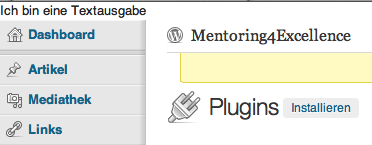
\includegraphics[angle={360}, scale=0.61]{pictures/printheader.png}
	    \caption{Printbefehl-Ausgabe}
	    \label{img:PRBEAUS}
	    	\end{center}
   \end{figure}
Dieses Verhalten ist darauf zurückzuführen, dass das Plugin nach dem aktivieren direkt geladen wird und so auf jede Seite vorhanden ist.\newline
Dies lässt sich durch das Hinzufügen von Funktionen unterbinden, welches in Listing \ref{VEBEBEI}, Zeile 8 - 10 dargestellt ist. 
\lstset{language={PHP},caption={Verbesserte Printausgabe},label=VEBEBEI}
\begin{lstlisting}
<?php
/*
Plugin Name: Mentoren-Suche - Printausgabe 2
Description: Ein zweiter Versuch
Version: 0.2
//...WEITERE ANGABEN VON INFORMATION-HEADER...
*/
function printausgabe(){
	print "Ich bin eine Textausgabe";
}
?>
\end{lstlisting} 
Das nun verwendete Plugin bewirkt, dass das Printstatement so isoliert wird, dass es erst bei unmittelbaren Aufruf verwendet wird. \newline
Zwar ist nach dem Aktivieren des Plugins das Textfeld verschwunden, allerdings taucht es dieses auch nicht an anderer Stekke auf. Dafür werden sogenannte Hooks (siehe Abschnitt \ref{sub_acvsfs}) verwendet.\footcitetgedr[Vgl.][Seite 38-39]{BB11} \newline
Bevor diese allerdings angesprochen werden und nach diesem kleinen Exkurs auch mit dem Mentoring-Plugin weitergearbeitet wird, wird im nächsten Kapitel \ref{subsub_debmod} noch die Aktivierung des Debug-Modus kurz erläutert.
\subsubsection{Debug-Modus}\label{subsub_debmod}
Es ist ratsam bei der Pluginentwicklung
 im sogenannten-Debug-Modus von Wordpress zu arbeiten, um so  Fehlermeldungen zu sehen und diese zu beheben.
Dieser Modus lässt sich in der Hauptkonfigurationsdatei \emph{wp-config.php} einstellen. Dafür muss im folgenden Listing der Wert in Zeile 9 von \emph{false} (ausgeschaltet) auf \emph{true} (eingeschaltet) geändert werden.\footcitetgedr[Vgl.][Seite 23]{BB11}
\lstset{language={PHP},caption={Debug-Modus aktivieren},label=CERPRAU}
\begin{lstlisting}
...
/**
 * For developers: WordPress debugging mode.
 *
 * Change this to true to enable the display of notices during development.
 * It is strongly recommended that plugin and theme developers use WP_DEBUG
 * in their development environments.
 */
define('WP_DEBUG', true);
...
\end{lstlisting} 
Nachdem der Debug-Modus aktiviert wurde, kann als Kontrolle nochmal die Funktion aus Listing \ref{CERPRAU} aktiviert werden. Anschließend wird zwar wieder im oberen Bereich die entsprechende Textausgabe ausgegeben, allerdings werden darunter einige Fehlermeldungen und Warnungen angezeigt: Der Debugger ist also aktiviert (siehe Abbildung \ref{img:PRMAKDE}). \newline
Wie dieser Fehler behoben wird ist an dieser Stelle schon aus Listing \ref{VEBEBEI} bekannt: Nämlich die Printausgabe als Funktion schreiben.\newline
 \begin{figure}[htbp]
	\begin{center}
		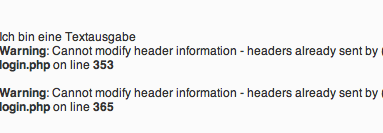
\includegraphics[angle={360}, scale=0.61]{pictures/printheadermeldung.png}
	    \caption{Printbefehl mit aktivierten Debugger}
	    \label{img:PRMAKDE}
	    	\end{center}
   \end{figure}\newline
Nachdem die Vorbereitungen abgeschlossen und die ersten Funktionen geschrieben wurde, wird nun das Referenzieren von Hooks über Filter und Actions angesprochen. 
\subsection{Hooks}\label{sub_acvsfs}
In diesem Kapitel wird sich mit sogenannten \emph{Hooks} beschäftigt. Diese sind dafür verantwortlich, wann ein Plugin ausgeführt ist. 
Genauer gesagt handelt es sich bei einem Hook um eine Art Eventhandler: Wenn ein bestimmtes Ereignis auftritt, wird eine gewisse Funktion ausgeführt. Ein solches Ereignis könnte beispielsweise vorliegen, wenn ein bestimmtes Menü angeklickt wird oder ein Suchfeld aktiviert wird.\newline
Dabei sollte noch erwähnt werden, dass sich diese Eventhandler in zwei Komponenten unterteilen lässt:Action- und Filter-Hooks.\footcitetgedr[Vgl.][Seite 39]{BB11}\newline
Wie diese genau funktionieren und allgemein aufgebaut sind, wird in den nächsten Abschnitten erläutert.

\subsubsection{Referenzieren mittels add\_action() und add\_filter()}\label{refmitaddacunaddfilt}
Bevor die eigentlichen Anwendungsbeispiele kommen, soll an dieser Stelle zuvor die allgemeine Syntax von \emph{action-} und \emph{filter}-Hooks erläutert werden:
\begin{table}[ht]
\centering
\begin{tabular}[h]{|l|c|c|c|c|c|}
\hline
\textbf{Hook-Art} & \textbf{Syntax} \\
\hline
Action & add\_action('Event','Funktion') \\
Filter & add\_filter('Event','Funktion') \\
\hline
\end{tabular}
\caption{Vergleich Action- und Filter-Hooks}
\label{tab:vglactufilhooks}
\end{table}
Anhand von Tabelle \ref{tab:vglactufilhooks} lässt sich erkennen, dass die beiden Hook-Arten genau gleich aufgebaut sind. Wie immer steckt hier der Teufel im Detail - genauer gesagt: Wie Wordpress mit diese beide Arten umgeht.\newline
Wenn eine Funktion zu einem Action-Hook verbunden wird, ignoriert die Funktion Eingabeparameter wie beispielsweise übergebene Variablen. Auch wenn die Funktion einen Rückgabewert besitzt, wird auch dieser Wert ignoriert.\footcitetgedr[Vgl.][Seite 40]{BB11} \newline
Dies ist der Punkt, an dem der Unterschied zum Filter-Hook klar wird: Dieser akzeptiert Eingabeparameter und Werte und kann diese verändert - oder eben gefiltert - zurückgeben.\newline
 Dies geschieht noch bevor dieser Parameter dem Benutzer auf dem Bildschirm angezeigt oder in die Wordpress-Datenbank geschrieben wird\footcitetint[Vgl.][]{MMTPA12}.\newline
 Im Grunde genommen haben die beiden Funktionen eines gemeinsam: Beide binden eine Event an eine Funktion, gehen nur jeweils anders damit um.\footcitetgedr[Vgl.][Seite 40]{BB11}\newline
  Eine überschaubare Funktionsreferenz von Action und Filter-Hooks lässt sich unter \url{http://codex.wordpress.org/Plugin_API} finden.
  
 \subsubsection{Hook-Anwendungsbeispiele}
 An dieser Stelle werden nun ein paar Beispiele aus dem Mentoren-Plugin genommen und weitestgehend erläutert. Anschließend wird noch eine weitere Funktion vorgestellt: Der add\_option-Hook.
\paragraph{Vordefinierte Actions}\ \newline
Wordpress bietet von Hause aus schon vordefinierte Actions, welche ab Wordpressversion 2.1 vorhanden und verwendbar sind. Da die Anzahl dieser vordefinierten Actions ziemlich umfangreich ist, wird an dieser Stelle nur auf ein Action verwiesen, welches vergleichbar oft in dem Mentorenplugin vorkam: Die Action \emph{add\_action}.\footcitetint[Vgl.][]{MMTPA12}

\lstset{language={PHP},caption={Beispiele für add\_action()},label=CADAC}
\lstset{
 morekeywords={add_action}
}
\begin{lstlisting}
<?php
...
add_action('admin_menu', 'register_Mentees_menu');
...
<?
\end{lstlisting}
An dieser Stelle wird auf die in Listing \ref{CADAC} vorgestellten Funktionen genauer eingegangen. \newline
Allgemein lässt sich formulieren, dass die Action \emph{admin\_menu} dafür verwendet wird, um ein zusätzliches Untermenü und bestimmte Menü-Optionen im Administrator-Bereich anzulegen.\footcitetint[Vgl.][]{MMTAR12}
Dies bedeutet, dass beim Aktivieren des Plugins verschiedene Actions ausgeführt werden. Beispielsweise wird eine Funktion \emph{register\_Mentees\_menu} aufgerufen, welche für die Erstellung des Submenüs zur Verwaltung des Plugins geschrieben wurde. \newline
Weitere Informationen werden zu diesem Thema im Kapitel \ref{Formular} angesprochen.

\paragraph{Eigene Actions}\ \newline
Natürlich ist es auch möglich eigene Actions zu schreiben und diese einer Menüstruktur zuordnen. Im Listing \ref{CADAC} sind solche Beispiele aufgelistet.
\lstset{language={PHP},caption={Beispiele für eigene add\_action()},label=CADAC}
\lstset{
 morekeywords={add_action}
}
\begin{lstlisting}
<?php
...
//wenn check erfolgreich, werden DB-Tabellen angelegt
add_action('hk_mentees_db_create','mentees_db_create');
add_action('hk_mentor_db_create','mentor_db_create');
...
<?
\end{lstlisting}
Falls also ein Mentor oder Mentee angelegt werden soll, werden die entsprechenden Daten wie Vor- oder Nachname in ein Formular eingetragen. Anschließend wird mit einem Button die Eingabe bestätigt. Genau das ist der Zeitpunkt, an dem die Action eintritt: Es muss eine Datenbank angelegt werden. Dies geschieht über die beiden Funktionen \emph{mentor\_db\_create} und \emph{mentees\_db\_create}. \newline
Wie mit solchen Datenbankobjekten interagiert wird, wird genau in Kapitel \ref{DBzugriff} besprochen.
\paragraph{Vordefinierte Filter}\ \newline
Da in dem aktuellen Plugin der Mentoren-Suche keine Filter zum Einsatz kommen, aber trotzdem für ein solches Tutorial von Bedeutung sind, wird an dieser Stelle auf Fachliteratur zurückgegriffen und entsprechend erläutert. \newline
Wie schon erläutert, handelt es sich bei Filter-Hooks um Funktionen, damit Wordpress bestimmte Text oder weitere Typen modifizieren kann.\newline
Nach Bondari und Griffiths\footcitetgedr[Vgl.][Seite 42 - 43]{BB11} soll das Ziel dieses kleinen Beispiel-Plugins nur verdeutlichen, wie Actions im Zusammenhang mit Filtern funktionieren. Dafür wird eine Kopie des Standard-Plugins \emph{hello dolly von Wordpress} verwendet und verändert. \newline
Die dazugehörige Plugindatei liegt im Pluginverzeichnis von Wordpress und lautet \emph{hello.php}
\lstset{language={PHP},caption={Beispiele für add\_filter()},label=CADFI}
\lstset{
 morekeywords={add_filter}
}
\begin{lstlisting}
<?php
...
//VORHER
add_filter('admin_footer','hello_dolly');

//NACHER
add_filter('the_content','hello_dolly');
...
<?
\end{lstlisting}
Wie in Listing \ref{CADFI} dargestellt, wird als Vorbereitung das Event von \emph{admin\_footer} auf \emph{the\_content} geändert, da hier die bisherigen Posts verändert werden sollen.\newline
Dafür wird in der Datei \emph{hello.php} zusätzlich auch die Funktion \emph{hello\_dolly()} verändert. \newline
Dies ist in Listing \ref{CAHD} genauer dargestellt.
\lstset{language={PHP},caption={Funktion \emph{hello\_dolly} mit Input-Variable},label=CAHD}
\lstset{
 morekeywords={add_filter}
}
\begin{lstlisting}
<?php
...
//VORHER
function hello_dolly() {
	$chosen = hello_dolly_get_lyric();
	echo "<p id='dolly'>$chosen</p>";
}

//NACHER
function hello_dolly($input) {
	$chosen = hello_dolly_get_lyric();
	return $input . "<p id='dolly'>$chosen</p>";
}
...
<?
\end{lstlisting}
Was hier nun passiert, lässt sich wie folgt beschreiben: Die Variable \emph{\$input} beschreibt den Inhalt eines jeden Posts. Dieser wird anschließend in die Filter-Funktion übertragen, modifiziert und anschließend per \emph{return} zurückgegeben.\newline
Anstatt die kompletten Inhalt eines Posts zu überschreiben, wird stattdessen ein beliebiger Text unterhalb des Posts eingebunden. Damit wird also schlussendlich der Inhalt verändert und dargestellt - genau das, was eine Filter-Funktion machen sollte.\newline
Unterm Strich lässt sich formulieren, dass eine Funktion, die bei einer Action aktiviert wird, keine Eingabe- und Ausgabewerte akzeptiert. \newline
Eine Action, die über eine Filter-Funktion aufgerufen wird, erlaubt die oben genannten Einschränkungen. Dies ist zugleich der Unterschied zwischen diesen beiden Event-Typen.\footcitetgedr[Vgl.][Seite 43]{BB11}
Weitere Informationen finden sich unter den folgenden Internetseiten zu finden:
\begin{enumerate}
	\item \url{http://codex.wordpress.org/Function\_Reference}
	\item \url{http://codex.wordpress.org/Action\_Reference}
\end{enumerate}
\paragraph{Funktion add\_option}\ \newline
Zum Schluss dieses Kapitels wird sich noch mit dem \emph{add\_option}-Hook beschäftigt. Dieser ist mehrmals im Plugin zum Einsatz gekommen und ist syntaktisch auch anders aufgebaut als ein \emph{filter} oder \emph{action}-Hook.\newline
Laut Mullenweg\footcitetint[Vgl.][Artikel Function Reference/add option]{MMTFR12} wird eine add\_option-Funktion dafür verwendet, um Optionen in die Wordpress-Datenbank zu schreiben.
Als erstes wird dabei geprüft, ob eine Funktion mit demselben Namen schon vorhanden ist. In diesem Fall wird ein \emph{false}  zurückgegeben.\newline
Wenn anschließend der Name keiner der geschützten Optionen überschreiben soll, wird die Option erstellt. Dies ist der allgemeine Ablauf, der sich hinter \emph{add\_option} befindet. Die allgemeine Syntax sowie ein Anwendungsbeispiel lässt sich aus Listing \ref{CADOP} ablesen.\newline
\lstset{language={PHP},caption={Beispiele für add\_option()},label=CADOP}
\lstset{
 morekeywords={add_option}
}
\begin{lstlisting}
<?php
...
//Allgemeine Syntax 
add_option('Option','Value','Deprecated','autoload')
//Beispiel
add_option('ms_frontend_searchform_url','','',yes);

<?
\end{lstlisting}
In dem in Listing \ref{CADOP} dargestellten Beispielen muss ergänzt werden, dass die Werte \emph{Value} (für Option-Name reserviert), \emph{deprecated} (nur für Wordpressversion 2.3) und \emph{autoload} (ob die Funktion automatisch geladen werden soll mit Standardwert \emph{yes} für ja) optional sind.\newline
Im konkreten Anwendungsbeispiel wird also die Option \emph{ms\_frontend\_searchform\_url} aufgerufen und in die Datenbank eingetragen. Diese Option ist dafür verantwortlich, dass im Frontendbereich an der Stelle, an dem der Shortcode eingebunden wird (ausführlich im nächsten Kapitel), eine Suchmaske erscheint und ausgeführt werden kann.\newline
Wie diese aussieht, wird im nächsten Kapitel näher besprochen.\newline
Soviel zu den Hooks. Im nächsten Kapitel \ref{shortcodes} wird die Thematik \nameref{shortcodes} behandelt.
\newpage
%%
%%%%********************************************************************************
\section{Menüerstellung}
Nachdem im vorigen Kapitel der allgemeine Aufbau eines Plugins und der Begriff des \emph{Hooks} erklärt und mit Beispielen aus der Mentoren-Suche erläutert wurde, geht es in diesem Kapitel um das erstellen einer Menüstruktur im Backend von Wordpress.\newline
Dabei wird zuerst auf den Begriff eines Menüs eingegangen (vgl. Abschnitt \ref{wasisteinmenue}), danach wird erläutert wie Menüs erstellt werden (vgl. Abschnitt \ref{ersttlm} und \ref{erstum}). Diese beiden Abschnitte werden dann mit Beispielen aus der Mentoren-Suche jeweils abgerundet (vgl. Abschnitt \ref{bsptlm}) und Abschnitt \ref{bsperstum}). Zum Schluss kommt dann noch ein Teil, der sich mit der Integration von Menüs in bestehende vom Wordpress-Backend beschäftigt (siehe Abschnitt \ref{integration}).
\subsection{Wozu dient ein Menü?}\label{wasisteinmenue}
Ein Menü dient zur Verwaltung des Plugins und ist im Backend zu finden. Dabei können beispielsweise verschiedene Optionen eingestellt werden können. Dabei kann Wordpress mit zwei verschiedenen Arten von Menüs umgehen. Dieses ist zum einen das Top-Level-Menü (siehe Abschnitt \ref{ersttlm}) und das Submenü (vgl. Abschnitt \ref{erstum}).\footcitetgedr[Vgl.][Seite 59]{BWPWP11}
\subsection{Erstellen von Top-Level-Menüs}\label{ersttlm}
Ein Top-Level-Menü - oder auch Obermenü - ist laut Williams/Richard/Tadlock\footcitetgedr[Vgl.][Seite 60 - 61]{BWPWP11} die oberste Einheit eines Menüs. Beispielsweise wäre das Menü \emph{Einstellungen} im Wordpress-Admin-Bereich ein Top-Level-Menü. Die Autoren raten, für jedes Plugin ein solches Menü zu erstellen, welche mehrere Einstellungsmöglichkeiten bietet.
Für die Erstellung eines Top-Level-Menüs wird die Funktion \emph{add\_menu\_page} verwendet\footcitetint[Vgl.][]{MMTADMPA13}:
\lstset{language={PHP},caption={Syntax der Top-Level-Menü - Funktion},label=BSPSYNTLMFUNWP}
\lstset{
 morekeywords={function,do_action,global,\$exit_msg}
}
\begin{lstlisting}
<?php 
...
  add_menu_page( $page_title, $menu_title, $capability, $menu_slug, $function, $icon_url, $position ); 
...
?>
\end{lstlisting}
Dabei sind die Parameter wie folgt zu verstehen:
\begin{enumerate}
	\item \textbf{\$page\_title}
	\begin{itemize}
		\item Dies ist der Titel der Seite und verpflichtend  (vom Typ String)
	\end{itemize}
	\item \textbf{\$menue\_title}
		\begin{itemize}
		\item Hierbei handelt es sich um den Menünamen (als String), welchem im Dashboard angezeigt werden soll. Auch dieser ist verpflichtend.
	\end{itemize}
	\item \textbf{\$capability}
	\begin{itemize}
		\item Dies ist die Beschreibung für die Fähigkeit an Rechten, um auf das Menü zugreifen zu können. Auch hierbei handelt es sich um einen String. Rechte sind hierbei als Rollen zu betrachten, mit denen ein Benutzer etwas im Blog ändern darf oder nicht. Dies ist von dem jeweiligen Recht abhängig. Weitere Informationen finden sich unter \url{http://faq.wpde.org/welche-benutzerrolle-bietet-welche-rechte}.
	\end{itemize}
	\item \textbf{\$menu\_slug}
	\begin{itemize}
		\item  Dies ist ein Bedienungsparameter, um die Einstellungsseite auf der Menüseite anzueigen. Es könnte also auch eine PHP-Datei sein. Dieser Parameter ist erforderlich.
	\end{itemize}
	\item \textbf{\$function}
	\begin{itemize}
		\item Ist der erste optionale Parameter, welcher eine Funktion angeben kann, die auf der aufzurufenden Seite ausgeführt werden soll.
	\end{itemize}
	\item \textbf{\$icon\_url}
	\begin{itemize}
		\item Die Icon-URL ist auch ein optionaler Parameter, mit dem der Programmierer die Möglichkeit hat, ein Menüicon einzubinden. Beispielsweise könnte dies bei einem professionellen Plugin durchaus Sinn machen (beispielsweise das Firmenlogo).
	\end{itemize}
	\item \textbf{\$position}
	\begin{itemize}
		\item Dieser optionale Parameter, der als Integer-Wert angegeben werden muss, beschreibt die Position, an der das Menü erscheinen soll. Je nach Zahl, wird das Menü dann an entsprechender Stelle eingeblendet. Wenn keine Zahl angegeben wurde, wird das Menü automatisch am Ende des Menüs angezeigt.
		\item Beispiele für Menüplatzierungen
		\begin{enumerate}
			\item 2 - Dashboard
			\item 20 - Seiten
			\item 65 - Plugins
			\item 70 - Benutzer
		\end{enumerate}
	\end{itemize}
\end{enumerate}
Wie in der oben genannten Aufzählung beschrieben, gibt es verschiedene optionale und verpflichtende Parameter. Um diese in der Praxis zu sehen, wird nun in Unterabschnitt \ref{bsptlm} ein Beispiel zu dieser Funktion vorgestellt und erläutert.
\subsubsection{Beispiel Top-Level-Menüs aus Mentoren-Suche}\label{bsptlm}
Nachdem die Theorie über das Erstellen von Top-Level-Menüs im Abschnitt \ref{ersttlm} besprochen wurde, wird nun anhand von einem Beispiel dieses Wissen praxisnah aufgezeigt. Dabei handelt es sich um das Obermenü des Plugins Mentoren-Suche (siehe Listing \ref{BSPTOPLEVELMENUE}.\newline
\lstset{language={PHP},caption={Beispiel Mentoren-Suche Top-Level-Menü},label=BSPTOPLEVELMENUE}
\lstset{
 morekeywords={function,do_action,global,\$exit_msg}
}
\begin{lstlisting}
<?php 
...
function register_Mentees_menu() {
	add_menu_page(__('Mentoren Suche','mentoren-suche'), __('Mentoren Suche','mentoren-suche'),'unfiltered_html', 'mentees', 'ms_row_edit');
}
...
?>
\end{lstlisting}
Die Funktion \emph{register\_Mentees\_menu()} hat die Aufgabe, den Menüpunkt \emph{Mentoren Suche} als Top-Level-Menü in das Backend von Wordpress einzubinden. Dazu wird die Rechteklasse \emph{mentees} verwendet, welche eigens in Blog der Mentorinnen und Mentoren erstellt wurde - also gewissermaßen eine selbst definierte Benutzerrechtsklasse. Anschließend wird die Funktion \emph{ms\_row\_edit} aufgerufen, mittels welcher die Datensätze von Mentorinnen und Mentoren bearbeitet und gelöscht werden kann. Wie dies schlussendlich aussieht, ist in Abbildung \ref{img:ausgtlmfunk} abgebildet.
  \begin{figure}[htbp]
	\begin{center}
		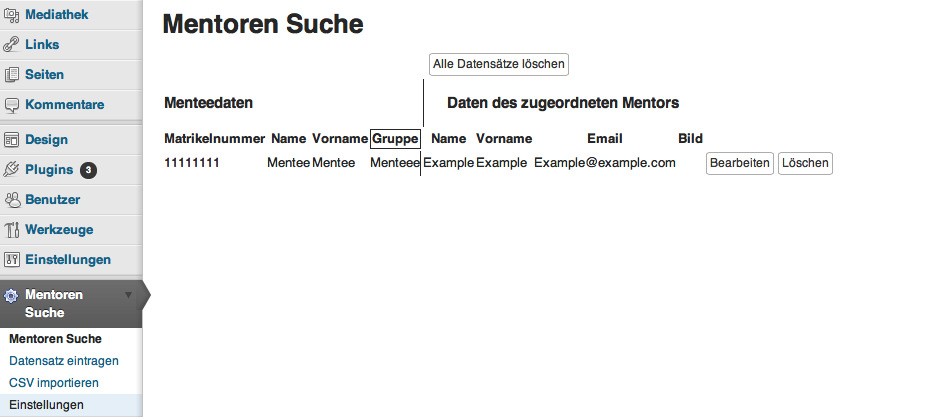
\includegraphics[angle={360}, scale=0.50]{pictures/mentsuchergmenue.png}
	    \caption{Ausgabe Top-Level-Menü-Funktion}
	    \label{img:ausgtlmfunk}
	    	\end{center}
   \end{figure}
\subsection{Erstellen von Submenüs}\label{erstum}
Da bereits im Abschnitt \ref{ersttlm} beschrieben wurde, wie Top-Level-Menüs zu erstellen sind, wird nun auf die Submenüs - oder auch Untermenüs - eingegangen.\newline
Beispielsweise, wäre laut Williams/Richard/Tadlock\footcitetgedr[Vgl.][61]{BWPWP11}  das Menü \emph{Allgemein} im Backend von Wordpress das Submenü, während \emph{Einstellungen} das Top-Level-Menü. \newline
Um ein solches Untermenü zu erstellen, wird die Funktion \emph{add\_submenu\_page} verwendet\footcitetint[Vgl.][]{MMTFRADSUBMP13} :
\lstset{language={PHP},caption={Syntax der Submenü - Funktion},label=BSPSBMFUNWP}
\lstset{
 morekeywords={function,do_action,global,\$exit_msg}
}
\begin{lstlisting}
<?php 
...
  add_submenu_page( $parent_slug, $page_title, $menu_title, $capability, $menu_slug, $function ); 
...
?>
\end{lstlisting}
Dabei sind die Parameter wie folgt zu verstehen:
\begin{enumerate}
	\item \textbf{\$parent\_slug}
	\begin{itemize}
		\item Hierbei handelt es sich einen nicht-optionalen Parameter, welcher den Namen des Obermenüs beschreibt. Falls ein Menü geschrieben werden soll, welches keinen Menü als Unterpunkt auftaucht, kann der Wert \emph{NULL} oder \emph{options.php} gesetzt werden.
	\end{itemize}
	\item \textbf{\$page\_title}
		\begin{itemize}
		\item Der Seitentitel beschreibt den Text, der auf der Seite als Titel nach dem anklicken des Submenüs angezeigt wird. Dieser ist in Form eines Strings zu verwenden und nicht optional.
	\end{itemize}
	\item \textbf{\$menu\_title}
	\begin{itemize}
		\item Der Menütitel beschreibt den Titel, welcher in dem Untermenü-Button angezeigt wird.
	\end{itemize}
	\item \textbf{\$capability}
	\begin{itemize}
		\item  Die \$capability beschreibt die Rechtezuteilung, damit User diese sehen oder nicht sehen können: Je nachdem, wie die Rechtevergabe aussieht. Diese Angabe ist nicht optional. Dabei kann zwischen verschiedenen Hierarchien von Rechten unterschieden werden. Diese fangen an oberster Stelle mit dem Super-Administrator und Administrator an, und hören bei dem Abbonennten auf. Weitere Informationen finden sich unter \url{http://codex.wordpress.org/Roles\_and\_Capabilities}.
	\end{itemize}
	\item \textbf{\$menu\_slug}
	\begin{itemize}
		\item  Dies ist Parameter, um das Menü eindeutig anzusprechen. Dies ist erforderlich, um das Elternmenü nicht mehrmals zu erstellen. Diese Angabe ist erforderlich.
	\end{itemize}
	\item \textbf{\$function}
	\begin{itemize}
		\item Hierbei handelt es sich um einen String in Form einer Funktion, welcher als Ausgabe für die angeklickte Seite dient. Dieser ist optional.
	\end{itemize}
\end{enumerate}
Die Theorie wird nun anhand eines Beispiels im Abschnitt \ref{bsperstum} erläutert.
\subsubsection{Beispiel Untermenü aus Mentoren-Suche}\label{bsperstum}
Die bereits genannten Parameter sollen nun anhand von einem Beispiel aus der Mentoren-Suche veranschaulicht werden. \newline
\lstset{language={PHP},caption={Beispiel Mentoren-Suche Submenü},label=BSPSUBMENUE}
\lstset{
 morekeywords={function,do_action,global,\$exit_msg}
}
\begin{lstlisting}
<?php 
...
function me_dataset_import() {
	add_submenu_page( 'mentees', __('Datensatz eintragen','mentoren-suche'), __('Datensatz eintragen','mentoren-suche'), 'unfiltered_html', 'row-import', 'ms_row_new');
}
...
?>
\end{lstlisting}
Die Funktion \emph{me\_dataset\_import} ist dafür da, den Untermenüpunkt \emph{Datensatz eintragen} in das Menü \emph{Mentoren Suche} einzubinden. Anschließend wird dann die Funktion \emph{row\_import}, welche dann die Funktion \emph{ms\_row\_new} aufruft. Diese ist zum Eintragen von Datensätzen vorhanden. Abschließend ist dieses Beispielmenü in der Abbildung \ref{img:aussub} dargestellt.
\newpage
  \begin{figure}[htbp]
	\begin{center}
		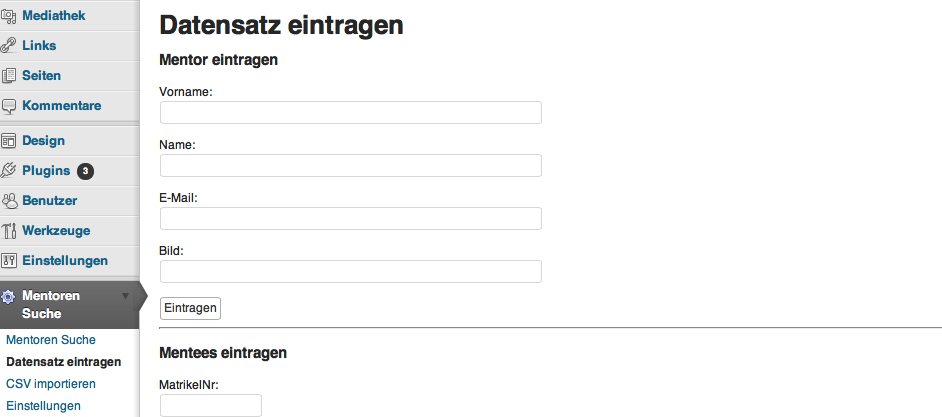
\includegraphics[angle={360}, scale=0.4]{pictures/mentsuchergsubmenue.png}
	    \caption{Ausgabe Submenü-Funktion}
	    \label{img:aussub}
	    	\end{center}
   \end{figure}
Im nächsten Kapitel geht es nicht um das neue anlegen von Top- oder Submenüs, sondern um die Integration von Menüs in bereits bestehende Standard-Menüs von Wordpress.
\subsection{Integration in bestehende Menüs}\label{integration}
Nachdem bereits erwähnt wurde, wie Top-Level- und Submenüs erstellt werden, kommt nun zum Schluss die Integration von Einstellungsseiten in eine vorhandene Menüstruktur.\newline
Wenn ein Plugin einen überschaubaren Umfang hat, besitzt es meistens auch nicht mehr als eine Einstellungsseite. Nun könnte ein Programmierer auch für diese Seite ein einzelnes Top-Level- und/oder Submenü erstellen. Alternativ dazu gibt es laut Williams/Richard/Tadlock\footcitetgedr[Vgl.][Seite 62]{BWPWP11} die Möglichkeit, bereits in vorhandenen Menüstrukturen, Untermenüs zu erstellen. Dies könnte je nach Kontext des Plugins beispielsweise unter Design oder Einstellungen eingebaut werden. Weitere Beispiele sind der Abbildung \ref{img:UEADWP} gezeigt.
  \begin{figure}[htbp]
	\begin{center}
		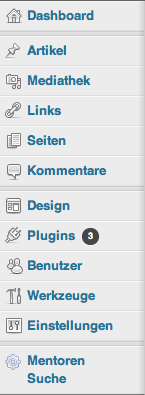
\includegraphics[angle={360}, scale=0.48]{pictures/dash.png}
	    \caption{Übersicht Admin-Bereich von Wordpress}
	    \label{img:UEADWP}
	    	\end{center}
   \end{figure}
\newpage Es gibt unter Wordpress sehr viele verschiedene Möglichkeiten, um die Standardmenüs mit eigenen zu erweitern. An dieser Stelle wird die Funktion \emph{add\_options\_page} verwendet. Die allgemeine Syntax sieht folgendermaßen aus\footcitetint[Vgl.][]{MMTADOPPA13}:
\lstset{language={PHP},caption={Syntax zum integrieren von Menüs in bereits vorhandene},label=BSPINTMENVOR}
\lstset{
 morekeywords={function,do_action,global,\$exit_msg}
}
\begin{lstlisting}
<?php
add_options_page( $page_title, $menu_title, $capability, $menu_slug, $function);
?> 
\end{lstlisting}
Im weiteren werden nun die einzelnen Parameter laut Wordpress Codex erläutert:
\begin{enumerate}
	\item \textbf{\$page\_title}
	\begin{itemize}
		\item Hierbei handelt es sich um einen Parameter vom Typ String und beschreibt den Titel der Seite, die beim auswählen des Menüs geöffnet wird. Diese Angabe nicht erforderlich.
	\end{itemize}
	\item \textbf{\$menu\_title}
		\begin{itemize}
		\item Auch dieser Parameter ist nicht optional und beschreibt den dargestellten Text für das Menü - also die Menübezeichnung. 
	\end{itemize}
	\item \textbf{\$capability}
	\begin{itemize}
		\item Der zweite Parameter beschreibt die Mindestfähigkeit an Rechten, um das Untermenü anklicken zu können. Auch hierbei handelt es sich im eine Rechte-Hierarchie, welche genauer unter der folgenden Adresse tiefer beschrieben wird: \url{http://codex.wordpress.org/Roles\_and\_Capabilities}.
	\end{itemize}
	\item \textbf{\$menu\_slug}
	\begin{itemize}
		\item  Hierbei handelt es sich um einen eindeutigen Indentifizierer, um das Untermenü eindeutig zu beschreiben. Auch dieser Parameter ist nicht optional.
	\end{itemize}
	\item \textbf{\$function}
	\begin{itemize}
		\item Hingegen den anderen Parametern, ist dieser Paramter optional und beschreibt eine Funktion, die aufgerufen wird, um den Inhalt der aufgerufenen Seite darzustellen.
	\end{itemize}
\end{enumerate}
Soweit an dieser Stelle zur Theorie. Im nächsten Unterabschnitt wird dann ein Beispiel gezeigt und erläutert.
\subsubsection{Beispiel Integration von Submenüs}
In diesem Beispiel, welches in Listing \ref{BSPHINUMVM} dargestellt ist, wird unter den Einstellungen im Dashboard von Wordpress ein weiteres Untermenü eingefügt.\footcitetgedr[Vgl.][Seite 62 - 63]{BWPWP11}
\lstset{language={PHP},caption={Beispiel hinzufügen eines Untermenüs zu vorhandenen Menüs},label=BSPHINUMVM}
\lstset{
 morekeywords={function,do_action,global,\$exit_msg}
}
\begin{lstlisting}
<?php
...
add_action( 'admin_menu', 'boj_menuexample_create_menu' );

function boj_menuexample_create_menu() {
	//create a submenu under Settings
	add_options_page( 'My Plugin Settings Page', 'Menu 	Example Settings', 'manage_options', __FILE__, 'boj_menuexample_settings_page' );
	}
...
<?
\end{lstlisting}
In diesem Beispiel wird ein Untermenü mit dem Namen \emph{My Plugin Settings Page} im Einstellungsmenü dargestellt (siehe Zeile 7). Anschließend wird der Seitentitel auch auf \emph{My Plugin Settings Page} gesetzt und die Mindestfähigkeit an Rechten auf manage\_options gesetzt (was soviel bedeutet, dass der Benutzer die Rechte haben muss, um die Einstellungen zu verändern / auf dieses Menü zugreifen zu können). Abschließend wird dann eine Funktion genannt, welche bei Aufruf des Menüs ausgeführt werden muss.\newline
Schlussendlich sieht dies dann folgendermaßen aus (siehe Abbildung \ref{img:untermenuinvorhmenu}):
  \begin{figure}[htbp]
	\begin{center}
		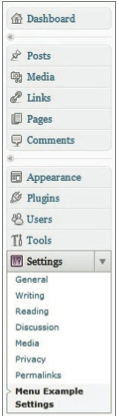
\includegraphics[angle={360}, scale=0.61]{pictures/untermenuinvorhmenu.png}
	    \caption{Eigenes Untermenü in vorhandene Menüstrukturen eingebunden}
	    \label{img:untermenuinvorhmenu}
	    	\end{center}
   \end{figure} \newline
Weitere Möglichkeiten, um Submenüs in Wordpress einzubinden sind beispielsweise\footcitetgedr[Vgl.][Seite 63]{BWPWP11}
\begin{enumerate}
\item add\_dashboard\_page - Fügt ein Untermenü zum Dashboard hinzu
\item add\_theme\_page - Fügt ein Untermenü zum Thememenü hinzu
\item add\_plugins\_page - Fügt ein Untermenü zum Pluginmenü hinzu
\end{enumerate}
Weitere sind unter der folgenden Adresse zu finden:\url{http://codex.wordpress.org/Administration\_Menus#Admin\_Menu\_Functions}\newline
Die Autoren Williams/Richard/Tadlock\footcitetgedr[Vgl.][Seite 63]{BWPWP11} raten an dieser Stelle dazu, wenn ein Plugin nur eine einzelne Einstellungsseite hat, diese als Untermenü in ein vorhandenes einzubinden. Wenn allerdings mehr als eines (wie beispielsweise bei der Mentoren-Suche der Fall), sollte ein eigenes erstellt werden.
\subsection{Ausblick} 
Insgesamt gibt es mehrere Möglichkeiten - je nach Bedarf - ein Menü neu anzulegen oder zu integrieren. \newline
Es sollte allerdings darauf geachtet werden, dass bei einer möglichen Veröffentlichung des Plugins auch in die Dokumentation gehört, wo die Plugineinstellungen gefunden werden können. Dies ist vor allem von großen Interesse, wenn neue Menüs in bestehende integriert werden.\footcitetgedr[Vgl.][Seite 60 - 61]{BWPWP11}
Weitere Informationen zu diesem Thema finden sich unter:
\begin{enumerate}
	\item \url{http://codex.wordpress.org/Function\_Reference} 	\item \url{http://codex.wordpress.org/Administration\_Menus}
	\item	\url{http://codex.wordpress.org/User\_Levels}
\end{enumerate}
\newpage
%%
%%%%********************************************************************************
\section{Shortcodes}\label{shortcodes}
In diesem Kapitel wird sich den Thema \emph{Shortcode} gewidmet. Dabei wird nach einer kleinen Definition, die Benutzung und der Einsatz in einer Wordpressumgebung erläutert. 
\subsection{Was ist ein Shortcode?}
Um Shortcodes zu verwenden, wird nun erläutert, um was es sich hierbei handelt. Nach Bondari und Griffiths
\footcitetgedr[Vgl.][Seite 177]{BB11} lässt sich ein Shortcode als Makro definieren, welches in einem Artikel oder Seite hinzugefügt werden kann. Damit lassen sich also bestimmte Funktionen zu einer Seite hinzufügen. \newline
Die offizielle technische Dokumentation von Wordpress\footcitetint[Vgl.][]{MMTSA12} bringt des weiteren noch hervor, dass ein Shortcode von einem Pluginentwickler dem eigentlichen Benutzer dabei hilft, auf einer bestimmten Seite - also im Frontend von Wordpress - das Plugin einzubinden.
\subsection{Shortcodes verwenden}
In Abbildung \ref{img:SHISEINB} ist der Shortcode für das Mentoren-Plugin abgebildet, welcher im Inhaltsbereich einer Seite / Artikel das Frontend der Mentorensuche einbindet - und zwar genau an der Stelle, an der er eingebunden wird.
   \begin{figure}[htbp]
	\begin{center}
	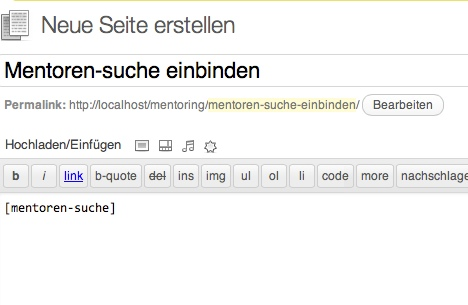
\includegraphics[angle={360}, scale=0.61]{pictures/shortcodeeinb.jpg}
	    \caption{Shortcode in Seite einbinden}
	    \label{img:SHISEINB}
	\end{center}
   \end{figure}\newline
Im Anschluss lässt sich die neue Seite (Abbildung \ref{img:shortcideeinber}) im Browser betrachten:
   \begin{figure}[htbp]
	\begin{center}
	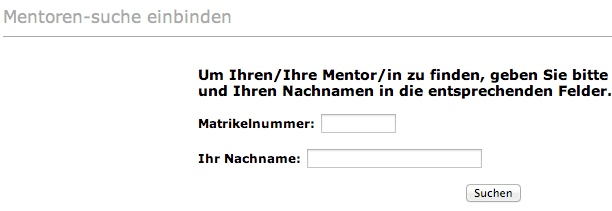
\includegraphics[angle={360}, scale=0.61]{pictures/shortcideeinber.jpg}
	    \caption{Ergebnis des eingebundenen Shortcodes}
	    \label{img:shortcideeinber}
	\end{center}
   \end{figure}
   \newpage
Wie ein solches Frontend erstellt wird, wird näher im Kapitel Formularerstellung (siehe Kapitel \ref{Formular}) erläutert. Hier geht es erstmal um die Einbindung solcher Funktionen.\newline
Schauen wir uns also an dieser Stelle genauer an, wie ein Shortcode erstellt ist. Die allgemeine Syntax ist in Listing \ref{CSHHIN} dargestellt. Der erste Teil beschäftigt sich mit der allgemeinen Syntax, anschließend ist ein Beispiel dargestellt. Dabei sollte diese Funktion in der Hauptdatei des Plugins vorhanden sein. Also beispielsweise \emph{mentoren-suche.php}.
\lstset{language={PHP},caption={Shortcode hinzufügen},label=CSHHIN}
\lstset{
 morekeywords={require_once,add_shortcode}
}
\begin{lstlisting}
<?php
...
// Allgemeine Syntax fuer einen Shortcode
add_shortcode('Shortcodename','AufzurufendeFunktion');
...

// Beispieldefinition des Shortcodes
require_once('frontend.php'); //frontend.php muss vorhanden sein
add_shortcode('mentoren-suche','showSearchArea');
...
?>
\end{lstlisting} 
Festzuhalten ist, dass Shortcodes sich ähnlich zu Filtern verhalten: Es werden Parameter akzeptiert und ein Ergebnis wiedergegeben. Dabei hat die \emph{add\_shortcode}-Funktion zwei Parameter: Einmal den Shortcodename, welcher dann in einem Post eingebunden werden kann (siehe \emph{mentoren-suche} und die aufzurufende Funktion \emph{showSearchArea}.\footcitetint[Vgl.][]{MMTSA12} \newline
an dieser Stelle soll auch ein kleiner Blick auf die Funktion \emph{showSearchArea} geworfen werden, um einen ersten Eindruck der Funktion zu bekommen. Diese ist (gekürzt) in Listing \ref{CSHFUNSSA} dargestellt.
\lstset{language={PHP},caption={Gekürzte Beispielfunktion showSearchArea},label=CSHFUNSSA}
\lstset{
 morekeywords={function,require_once,add_shortcode}
}
\begin{lstlisting}
/**
* Zeigt die Suchmaske fuer das Frontend an.
*/
function showSearchArea()
{ 
  //Variablendefinitionen
  
  if(isset($send_mentorenSearch))
  {
  ...
  		// Ausgabe des Ergebnisses
  		// Fehlermeldung: Eingabedaten sollten vervollstaedigt werden 	
  ... 
 }
 else{
   ...  
     // Eingabe der Matrikelnummer und des Nachnamens
   ...
 }
}
\end{lstlisting} 
Diese Funktion ist in der Datei \emph{frontend.php} vorhanden und dient dazu, ein Formular mit einer Suchfunktion darzustellen.Dabei wird geprüft, ob ein Ergebnis vorliegt - also falls der entsprechende Datensatz gefunden wurde. Falls keiner gefunden wurde, wird eine entsprechende Fehlermeldung ausgegeben. Zusätzlich erfolgt bei einer leeren Eingabe eine Meldung, dass Matrikelnummer und Nachname eingeben werden müssen und ein Link zur Suchformular verweist. Weitere Informationen für Shortcodes finden sich unter \url{http://codex.wordpress.org/Shortcode}. \newline
Im nächsten Kapitel geht es um die Wordpress \nameref{shapi}.
\subsection{Shortcode-API}\label{shapi}
Die Shortcode-\gls{API} wurde mit Wordpress 2.5 eingeführt und beinhaltet Funktionen, um spezielle Makros zum erstellen von Shortcodes in Posts zu verwenden.\newline
An dieser Stelle werden ausgewählte Funktionen vorgestellt und erläutert\footcitetint[Vgl.][]{MMTSA12}:
\begin{enumerate}
	\item {\bf function add\_shortcode(\$tag, \$func)} 
	\begin{itemize}
		\item Diese Funktion wurde bereits im Beispiel-Listing \ref{CSHHIN} verwendet und dient dazu, neue Shortcodefunkionen zu registrieren.
		\item Dabei ist \emph{\$tag} der Shortcodename, welcher der Benutzer in einem Post verwenden kann
		\item Der zweite Parameter \emph{\$func} dient dazu, eine bestimmte Funktion auszuführen, wenn der Shortcode aktiviert wird.
	\end{itemize}
	\item {\bf function remove\_shortcode(\$tag)} 
	\begin{itemize}
		\item Im Allgemeinen lässt sich hiermit ein Shortcode von einer Seite entfernen und es wird nur der Inhalt angezeigt, der auch ohne Shortcode vorhanden ist.
		\item Der Parameter \$tag entspricht hierbei dem Shortcodenamen, der von Benutzer verwendet wird (Parameter 1 in \emph{add\_shortcode})
		\item Beispielsweise lässt sich diese Funktion verwenden, wenn auf einer Seite ein oder mehrere Shortcodes eingebunden sind und eine davon temporär oder für immer deaktiviert werden soll, ohne das entsprechende Plugin zu deinstallieren.
	\end{itemize}
	\item {\bf function remove\_all\_shortcodes()} 
	\begin{itemize}
		\item Diese Funktion deaktiviert im Gegensatz zu \emph{function remove\_shortcode(\$tag)} alle Shortcodes auf einer Seite.
	\end{itemize}
	\item {\bf function do\_shortcode(\$content)} 
	\begin{itemize}
		\item Die Funktion do\_shortcode(\$content) eignet sich dazu, in einem Post andere Funktionen zusätzlich einzubinden. Beispielsweise könnte dies ein Kontaktformular sein.
	\end{itemize}
\end{enumerate}
Weitere Funktionen sind auf der offiziellen Shortcode-API seite von Wordpress zu finden (siehe \url{http://codex.wordpress.org/Shortcode\_API#Function\_reference})

\newpage
%%
%%%%********************************************************************************
\section{Datenbankzugriff über Plugin-API}\label{DBzugriff}
In diesem Kapitel geht es um die Interaktion zwischen Datenbank und Plugin. Es wird allgemein auf die entsprechende Datenbankschnittstelle sowie einigen Beispielen zur Manipulation und Ausgabe von SQL-Anweisungen eingegangen. Weiterhin wird darauf eingegangen, wie Angriffe auf die Datenbank verhindert werden können (vgl. Abschnitt \ref{verhsqlinj}).
\subsection{Die Datenbankschnittstelle WPDB}
Wordpress bietet eine Schnittstelle an, mit der Datenbanken angesprochen werden können. Diese heißt \emph{wpdb} - eine Abkürzung für \emph{Wordpress Database} - und basiert auf ezSQL.\footcitetint[Vgl.][Abschnitt Interfacing With the Database]{MMPQ12} \newline
Laut Vincent\footcitetint[Vgl.][]{JVEZSQL} ist ezSQL eine OpenSource Datenbankklasse, welche auf \gls{PHP} basiert und dazu dient, zwischen einem PHP-Skript und einer Wordpress-Datenbank zu interagieren.\newline
Grundvoraussetzung ist eine globales Objekt, über welche dann auf die Datenbank zugegriffen werden kann. Diese nennt sich \$wpdb und soll verhindern, dass Funktionen aus der WPDB-Klasse direkt aufgerufen werden können. Dies kann zu Kompatibilitätsproblemen führen und wird von Wordpress nicht unterstützt.\newline
Bevor sich den Möglichkeiten dieses Objektes zugewendet wird, werden noch zwei wichtige Informationen über die WPDB-Schnittstelle aufgezeigt. Zum einem kann diese Schnittstelle nur mit der Wordpress-Datenbank kommunizieren, zum anderen ist es manchmal auf notwendig mit anderen Datenbanken zu interagieren. \newline
Wenn mit einer anderen oder mehreren Datenbanken interagieren werden soll, ist das Plugin Hyperdb hilfreich. Dieses ist unter \url{http://wordpress.org/extend/plugins/hyperdb/} zu finden.\footcitetint[Vgl.][Abschnitt Notes On Use]{MMPQ12}\newline
In diesem Tutorial wird mit der Standard-Datenbank von Wordpress gearbeitet und somit muss kein zusätzliches Plugin verwendet werden. 
\subsubsection{Syntax und grundsätzliche Beispiele}\label{sygrbei}
Nachdem die Theorie soweit besprochen wurde, geht es nun um den Syntaxaufbau und die ersten Beispiele. \newline
Die allgemeine Syntax einer Abfrage an die Datenbank ist in Listing \ref{ANANDB1} dargestellt.
\lstset{language={PHP},caption={Allgemeine Syntax},label=ANANDB1}
\lstset{
 morekeywords={function,do_action,global,\$exit_msg,\$wpdb}
}
\begin{lstlisting}
<?php
...
$wpdb->query('query');
...
<?
\end{lstlisting}
Wie sich erkennen lässt, ist der erste Teil einer jeden Datenbankinteraktion immer das \$wpdb-Objekt. Gefolgt wird das Objekt von einem \emph{->}. Hierbei handelt es sich um einem Operator, welcher eine Methode aufruft. Dieser ist vergleichbar mit dem Punktoperator im objektorientierten Java. Anschließend wird die Funktion \emph{query} aufgerufen. Gefolgt von einem Datenbankbefehl, der in diesem Beispiel in Klammern und Hochkommata steht. Insgesamt sendet diese Anfrage einen Integer zurück, welcher beispielsweise die Anzahl der selektierten Zeilen zurückgibt. Wenn die Funktion einen Fehler enthält, wird automatisch ein \emph{FALSE}, also eine \emph{NULL} zurückgegeben.\footcitetint[Vgl.][Abschnitt Run Any Query on the Database]{MMPQ12} \newline
Soviel erstmal zum ersten Eindruck. In den nächsten Unterkapiteln geht es um einzelne SQL-Anweisungen und wie diese ausgeführt werden können. Anschließend wird im Kapitel \ref{beiamensuc} die Theorie mit Praxisbeispielen aus dem Plugin Mentoren-Suche abgerundet. 
\paragraph{SELECT von Variablen}\ \newline
Als erstes weiterführendes Beispiel, sollen bestimmte Variablen mittels einer SELECT-Anweisung aus der Datenbank ausgelesen werden.\newline
Dafür wird die sogenannte \emph{get\_var}-Funktion verwendet. Diese kann eine einzelne Variable aus der Datenbank zurückgeben. Sie eignet sich also perfekt für unsere oben erwähnte Anforderung. Wenn kein Ergebnis vorhanden ist, wird auch hier eine NULL zurückgegeben.\newline
Kommen wir an dieser Stelle nun zu dem Syntaxaufbau, welches in Listing \ref{SEEINVA} dargestellt ist. 
\lstset{language={PHP},caption={Selektion einer Variablen},label=SEEINVA}
\lstset{
 morekeywords={function,do_action,global,\$exit_msg,\$wpdb}
}
\begin{lstlisting}
<?php
...
$wpdb->get_var('query',column_offset,row_offset);
...
<?
\end{lstlisting}
Dieser Syntaxaufbau aus Listing \ref{SEEINVA} ist wie folgt zu beschreiben:
\begin{enumerate}
	\item {\bf query} 
	\begin{itemize}
		\item Bei \emph{query} handelt es sich um einen String, welcher ausgeführt werden soll. 
	\end{itemize}
	\item {\bf column\_offset}
	\begin{itemize}
		\item Ein Integerwert, welcher die gewünschte Spalte auswählt. Hierbei stellt der Wert 0 die erste Zeile dar und ist auch gleichzeitig der Initalisierungswert.
	\end{itemize}
	\item {\bf row\_offset}
	\begin{itemize}
		\item Hierbei handelt es sich um einem String oder integer, welcher die gewünschte Zeile angibt. Auch hier ist der Initalisierungswert 0 und stellt die erste Zeile dar. 
	\end{itemize}
\end{enumerate}
Die Informationen wurden aus der offiziellen Wordpress-API genommen und entsprechend aufbereitet.\footcitetint[Vgl.][SELECT a Variable]{MMPQ12} Im nächsten Abschnitt geht es um das Selektieren von Zeilen.
\paragraph{SELECT von Zeilen}\label{SELEZEI}\ \newline
Um eine Zeile in einer SELECT-Abfrage einzubinden, wird die Funktion \emph{get\_row} verwendet. Diese kann eine Zeile als einzelnes Objekt oder als Array wiedergeben. Wenn mehr als eine Zeile zurückgegeben wird, wird nur die erste ausgewählte Zeile ausgebenden - die anderen allerdings im Zwischenspeicher für den späteren Gebrauch gespeichert. Falls kein Ergebnis gefunden wird, wird auch hier eine \emph{NULL} zurückgegeben wird.\footcitetint[Vgl.][SELECT a Row]{MMPQ12} Um diese Theorie zu verdeutlichen, wird nun die Syntax erläutert. 
\lstset{language={PHP},caption={Selektion einer Zeile},label=SELEINZEI}
\lstset{
 morekeywords={function,do_action,global,\$exit_msg,\$wpdb}
}
\begin{lstlisting}
<?php 
...
$wpdb->get_row('query', output_type, row_offset); 
...
?> 
\end{lstlisting}
Gehen wir nun auf die einzelnen Syntaxelemente ein:
\begin{enumerate}
	\item {\bf query}
	\begin{itemize}
		\item Auch hier handelt es sich wieder um einen String, der ausgeführt werden soll.
	\end{itemize}
	\item {\bf output\_type }
	\begin{itemize}
		\item Hier gibt es drei vordefinierte Konstanten, von denen jeweils eine eingesetzt werden darf. 
		\begin{enumerate}
			\item Objekt: Ergebnis wird als Objekt wiedergegeben
			\item Array\_A: Ein assoziatives (also mit nichnumerischen Schlüsseln) wird zurückgegeben
			\item Array\_N: Ein nummerisches Array wird zurückgegeben (also mit numerischen Schlüsseln)
		\end{enumerate} 
	\end{itemize}
	\item {\bf row\_offset }
	\begin{itemize}
		\item Bezeichnet die gewünschte Zeile. Auch hier ist die Initialisierungswert \emph{NULL} und stellt zugleich die erste Zeile dar. 
	\end{itemize}
\end{enumerate}
Im nächsten Abschnitt wird das selektieren von Spalten besprochen.
\paragraph{SELECT von Spalten}\ \newline
Um Spalten zu selektieren, gibt es die Funktion \emph{get\_col}, welche ein Array ein Array der ausgewählten Spalten zurückgibt. Bei einem nicht vorhandenem Ergebnis leeres Array zurückgegeben.\footcitetint[Vgl.][SELECT a Column]{MMPQ12} Die Syntax lautet folgendermaßen:
\lstset{language={PHP},caption={Selektion von Spalten},label=SELVOSP}
\lstset{
 morekeywords={function,do_action,global,\$exit_msg,\$wpdb}
}
\begin{lstlisting}
<?php 
...
$wpdb->get_col('query',column_offset); 
...
?> 
\end{lstlisting}
Es handelt sich hierbei um eine relativ kleine Syntax, welche nun im Detail besprochen wird:
\begin{enumerate}
	\item {\bf query}
	\begin{itemize}
		\item So wie bei den oben genannten Formen, handelt es sich hier auch um den auszuführenden String.
	\end{itemize}
	\item {\bf column\_offset}
	\begin{itemize}
		\item Der column\_offset bezeichnet die ausgewählte Spalte in Form eines Integers und wird mit NULL initialisiert.
	\end{itemize}
\end{enumerate}
Soviel zu den Select-Befehlen. Nun wird auf zwei weitere Abfragen eingegangen; nämlich \nameref{insert} und \nameref{update}.
\paragraph{INSERT von Spalten}\label{insert}\ \newline
Für das Einfügen von Spalten bieten sich in der wpdb-Umgebung die Funktion \emph{insert} an. Diese besteht aus drei Parametern und wird nun anhand der Syntax erläutert\footcitetint[Vgl.][INSERT rows]{MMPQ12} :
\lstset{language={PHP},caption={Insert von Spalten},label=INVOSP}
\lstset{
 morekeywords={function,do_action,global,\$exit_msg,\$wpdb}
}
\begin{lstlisting}
<?php 
...
$wpdb->insert( $table, $data, $format ); 
...
?> 
\end{lstlisting}
Soviel zum allgemeinen Syntaxaufbau. Die einzelnen Elemente bedeuten dabei folgendes: 
\begin{enumerate}
	\item {\bf \$table}
	\begin{itemize} 
		\item Der Name der Tabelle, in die Daten eingefügt werden sollen. Dieser erste Parameter wird in Form des Typs \emph{String} angegeben.
	\end{itemize}
	\item {\bf \$data}
	\begin{itemize}
		\item Beschreibt die konkreten Daten, die eingefügt werden sollen. Dabei handelt es sich um ein Objekt vom Typ \emph{array}	
	\end{itemize}
	\item {\bf \$format}
	\begin{itemize}
		\item Dies ist eine optionale Angabe, die für  das Format aus \$data steht. Das bedeutet, wenn in \$data nur Strings stehen, kann hier \%s gesetzt werden und alle Inhalte werden als Strings behandelt. Hiermit lässt sich der genaue Inhalt von \$data angeben.
	\end{itemize}
\end{enumerate}
\paragraph{UPDATE von Spalten}\label{update}\ \newline
Der letzte der SQL-Anweisungen, der hier vorgestellt wird, ist der Update-Befehl\footcitetint[Vgl.][UPDATE rows]{MMPQ12}. Dieser eignet sich dafür, eine Zeile zu verändern. Dabei gibt der Befehl ein \emph{false} bei einem aufgetretenen Fehler zurück.\newline
Die allgemeine Syntax lässt sich wie folgt beschreiben:
\lstset{language={PHP},caption={Update von Spalten},label=UPVOSP}
\lstset{
 morekeywords={function,do_action,global,\$exit_msg,\$wpdb}
}
\begin{lstlisting}
<?php 
...
$wpdb->update( $table, $data, $where, $format = null, $where_format = null ); 
...
?> 
\end{lstlisting}
\begin{enumerate}
	\item \textbf{\$table}
	\begin{itemize}
		\item Auch hier ist mit dieser Anweisung die Tabelle gemeint, auf die sich bezogen wird.
	\end{itemize}
	\item \textbf{\$data}
	\begin{itemize}
		\item Auch hier handelt es sich um die Daten, die verändert werden sollen.
	\end{itemize}
	\item \textbf{\$where}
	\begin{itemize}
		\item Bei der where-Angabe handelt es sich um eine spezielle Anweisung, was in einer Spalte oder Zeile geändert werden soll. Hier ist es auch möglich, mehrere Angaben mit dem logischen AND zu verknüpfen.
	\end{itemize}
	\item \textbf{\$format}
	\begin{itemize}
		\item format beschreibt die Art der ausgewählten Daten - genauer gesagt um welchen Datentypen es sich handelt. Bei einem String würde ein \%s angegeben werden und alle Inhalte wie Strings behandelt. Diese Angabe ist optional.
	\end{itemize}
	\item \textbf{\$where\_format}
	\begin{itemize}
		\item Auch hierbei handelt es sich um eine optionale Angabe, welche beschreibt, welche Art von Format für den Update-Befehl ausgewählt werden soll. Auch diese Angabe ist optional und für einen String für \%s dienen und alle anderen Datentypen ignoriert werden.
	\end{itemize}
\end{enumerate}
Weitere Informationen befinden sich unter der Adresse \url{http://codex.wordpress.org/Class_Reference/wpdb}. Hier sind auch einige Beispiele vorhanden. Konkrete Beispiele aus dem Mentoren-Plugin finden sich hingegen im nächsten Kapitel \ref{beiamensuc}.
\subsubsection{Beispiele aus dem Plugin Mentoren-Suche}\label{beiamensuc}
Nachdem in Kapitel \ref{sygrbei} einige Befehle angesprochen wurden, werden diese nun anhand von Praxisbeispielen aus dem Plugin \emph{mentoren-suche}  vorgestellt und erläutert. Dabei wird nun so vorgegangen, dass zuerst ein Beispiel genannt, welches im Anschluss erläutert wird.
\paragraph{Beispiel SELECT von Zeilen}\ \newline
Eine normale SELECT-Anfrage stellt die einfachste aller Anfragen dar. Dieser soll einen bestimmten Inhalt aus der Datenbank auslesen. Dabei kommt der SELECT-Befehl zum Einsatz (siehe dazu \ref{SELEZEI}).\newline
In dem in Listing \ref{SELSPMP} dargestellten Auszug aus der Funktion \emph{ms\_showDeleteDataForm()}, welche für  das Anzeigen eines Datensatzes für das Löschen-Formulars (näheres zu Formulare in Kapitel \ref{Formular}) programmiert wurde, besteht aus 2 Teilen. \newline
\lstset{language={PHP},caption={Beispiel SELECT von Zeilen aus mentoren-plugin},label=SELSPMP}
\lstset{
 morekeywords={function,do_action,global,\$exit_msg,\$wpdb}
}
\begin{lstlisting}
<?php
...
function ms_showDeleteDataForm()
{

    $sql_mentorID="SELECT mentees_mid ".
                  "FROM ".MENTEE_TABLE.   
                  " WHERE mentees_matrikelnr ='".
                  $delete_mentee_id."'";
    $rs_mentorID=$wpdb->get_row($sql_mentorID);
}
...
<?
\end{lstlisting}
Der erste Teil definiert einen Befehl zum selektieren eines bestimmten Datensatzes, der zweite in Zeile 10 dargestellte Befehlt gibt dann das Ergebnis wieder. Dieses kann dann mit der Variable  \emph{\$rs\_ mentorID} weiter verwendet werden.\newline
Der Befehl wurde entsprechend verschachtelt, um potenzielle SQL-Injections zu vermeiden. Näheres dazu unter Abschnitt \ref{verhsqlinj}
\paragraph{Beispiel SELECT von Spalten}\ \newline
Im Mentoren-Plugin wurden keine Abfragen zum selektieren von Spalten verwendet. Deshalb wird an dieser Stelle auf das Beispiel aus dem offiziellen Wordpress-Codex verwiesen. Dieses ist unter
\begin{enumerate}
	\item \url{http://codex.wordpress.org/Class_Reference/wpdb#SELECT_a_Column}
\end{enumerate}
zu finden.
\paragraph{Beispiel INSERT von Spalten}\ \newline
Der INSERT-Befehl dient dem Einfügen von Spalten und besteht insgesamt aus 3 Parametern. Diese wurde bereits näher in Abschnitt \ref{insert} erläutert. 
\lstset{language={PHP},caption={Beispiel INSERT von Spalten aus mentoren-plugin},label=INSPMP}
\lstset{
 morekeywords={function,do_action,global,\$exit_msg,\$wpdb}
}
\begin{lstlisting}
<?php
...
function ms_m_data_insert() {

	global $wpdb;

if(!empty($_POST['ms_m_name']) && //...)
	{		
	  $name = $_POST['ms_m_name']; 
	  $vorname = $_POST['ms_m_vorname']; 
	  //...
	
	$rows_affected = $wpdb->insert(MENTOR_TABLE, array( 'mentoren_name' => $name, 'mentoren_vorname' => $vorname,... ) );
	
	} else {
		echo " //... Error ";
	}
...
<?
\end{lstlisting}
Der in Listing \ref{INSPMP} dargestellte Quellcode ist ein Teil der Funktion \emph{ms\_m\_data\_insert()}, welche dazu dient nach einem Submit-Button, die einzelnen Mentoren in die Mentoren-Tabelle der Datenbank zu speichern. Es handelt sich hierbei nur um ein gekürztes Beispiel, um sich auf den wesentlichen Inhalt zu konzentrieren. \newline
Im Grunde geht es darum, dass bei der Eingabe des Namen und Vornamen des Mentors in der Eingabemaske, dieser in die Datenbank eingetragen wird. \newline
Dafür wird in Zeile 13 die INSERT-Methode verwendet. Die betreffende Tabelle heißt MENTOR\_TABLE und die konkreten Daten werden mittels eines Arrays eingetragen. \newline
Zur Vollständigkeit wird an dieser Stelle angemerkt, dass falls die Eingabe des Mentors nicht korrekt ist, ein entsprechender Fehler (siehe Zeile 16) ausgegeben wird.
\paragraph{Beispiel DROP von Spalten}\ \newline
Da keine Update-Anweisung im Plugin Mentoren-Suche verwendet wurde, wird an dieser Stelle auf die offizielle Wordpress-Dokumentation verwiesen (siehe dazu \url{http://codex.wordpress.org/Class\_Reference/wpdb\#UPDATE\_rows}) \newline
Stattdessen wird aber kurz der Befehl zum Löschen von Tabellen vorgestellt: Der DROP-Befehl\footcitetint[Vgl.][How to Get Your WordPress Plugin To DROP TABLE From The Database]{MGDRTAPL}. \newline
Die in Listing \ref{CDRMP} verwendete Funktion dient dazu, das Plugin komplett zu löschen. Dabei wird - neben anderen kleineren Anweisungen - auch die Tabelle gelöscht. So wird nicht nur nach dem Deaktivieren, das Plugin aus dem Front- und Backend, sondern auch aus der Datenbank gelöscht.
\lstset{language={PHP},caption={Beispiel DROP-Anweisung aus mentoren-plugin},label=CDRMP}
\lstset{
 morekeywords={function,do_action,global,\$exit_msg}
}
\begin{lstlisting}
<?php
...
function pluginUninstall() {
	global $wpdb;
	
	//Tabellen loeschen:
  $sql = "DROP TABLE ".MENTOR_TABLE;

  $wpdb->query($sql);

  $sql = "DROP TABLE ".MENTEE_TABLE;
  $wpdb->query($sql);
}
...
?>
\end{lstlisting}
Was in diesem Ausschnitt nun passiert ist folgendes: Nachdem ein bereits erzeiugtes wpdb-Objekt zugeriffen wurde, wird in der Zeile 7 die Anweisung \emph{DROP\_TABLE} ausgeführt. Die allgemeine Syntax lautet: 
\begin{itemize}
	\item "DROP TABLE " .TABELLENNAME;
\end{itemize}
Diese bewirkt, dass die Tabelle \emph{MENTEE\_TABLE} gelöscht wird. In Zeile 12 wird die Anweisung dann schlussendlich ausgeführt. Soviel zu den Beispielen für die SQL-Anweisungen im Zusammenhang mit dem \emph{\$wpdb}-Objekt von Wordpress.\newline
Weitere Informationen werden unter den folgenden Internetadressen gefunden:
\begin{enumerate}
	\item \url{http://codex.wordpress.org/Class_Reference/wpdb}
\end{enumerate}
Im nächsten Kapitel werden noch in \ref{verhsqlinj} das Verhindern von SQL-Injections angesprochen.
\subsection{Verhindern von SQL Injections}\label{verhsqlinj}
In diesem Abschnitt wird erläutert, wie sich SQL-Injections in der Pluginentwicklung verhindern lassen. Dies ist das Thema dieses letzten Abschnitts des Kapitels \ref{DBzugriff}.\newline
SQL Injections bezeichnen einen Angriff auf eine SQL-Datenbank, indem SQL-Anfragen so manipuliert werden, dass Sie vertrauliche Daten ausspähen können. Es handelt sich also hierbei um eine Sicherheitslücke, welche aber mit bestimmten Anweisungen verhindert werden können.\footcitetint[Vgl.][SQL-Injection]{WIKSI12}\newline Diese werden an dieser Stelle vorgestellt.
Eine einfache und effektive Lösung, um solche Angriffe zu verhindern, ist es, SQL-Abfragen (zu Deutsch \emph{SQL-Abfragen}) mit der Prepare-Anweisung zu versehen. Diese Anweisung bereinigt und entgeht der eigentlichen SQL-Anweisung. \newline
Praktisch betrachtet, soll an dieser Stelle in Beispiel im Listing \ref{CVESQLINJBSP} aufgezeigt werden.
\lstset{language={PHP},caption={Beispiel für SQL-Injection-Verhinderung},label=CVESQLINJBSP}
\lstset{
 morekeywords={function,do_action,global,\$exit_msg}
}
\begin{lstlisting}
<?php

//1. Abfrage ohne prepare()-Statement
SELECT 'post_title'
FROM $wpdb->posts
WHERE 'post_author' = 1

//2. Abfrage mit prepare()-Statement in Datei 1
$sql = "SELECT 'post_title'
		FROM $wpdb->posts
		WHERE 'post_author' = %d";

//Datei 2 mit prepare()
<?php
	$id = 1;
	$safe_sql = $wpdb->prepare($sql,$id);
	$posts = $wpdb->getresults ($safe_sql);
?>

//EOF
?>
\end{lstlisting}
Dieses Beispiel gibt die Titel aller Autoren aus, welche die ID 1 haben. Die Abfrage wird dabei auf die Tabelle \emph{posts} bezogen.\newline
Nun zur Erläuterung: 
\begin{enumerate}
	\item Im ersten Beispiel ohne dem prepare-Statement, wird die SQL-Anweisung sozusagen im Klartext geschrieben: Es ist möglich, die Autoren-ID mitzulesen und entsprechend zu manipulieren.
	\item Im zweiten Beispiel wird anders verfahren. Die eigentliche SQL-Anweisung wurde mit Platzhaltern ausgestattet (siehe Zeile 11: \%d). \newline
	Im zweiten Teil dieses Beispiels wird von einer anderen \gls{PHP}-Datei auf die Anweisung zugegriffen. Dabei wir zuerst eine Variable vom Namen \%id angelegt und mit dem Wert 1 initialisiert. \newline
	Anschließend wird mittels des \emph{prepare}-Statements die Anweisung in Zeile 9 mittels \emph{\$sql} und \emph{\$id} aufgerufen.\newline
	Weiterhin wird dann mittels \emph{getresults} das Ergebnis der \$safe\_sql-Anfrage in \emph{posts} gespeichert und kann weiterverarbeitet werden.
\end{enumerate}
Der Vorteil an dem Prepare-Statement ist also, dass nur Vorlagen an Abfragen geschrieben werden, aber mittels entsprechender Variablen dynamisch verwendet werden können und so eine SQL-Injection nicht mehr so einfach möglich ist.\footcitetgedr[Vgl.][Seite 157 - 158]{BWPWP11} \newline
Wie dies genauer im Mentoren-Plugin aussieht, ist in Listing \ref{CVESQLINJ} dargestellt.
\lstset{language={PHP},caption={Verhindern einer SQL-Injection aus mentoren-suche},label=CVESQLINJ}
\lstset{
 morekeywords={function,do_action,global,\$exit_msg}
}
\begin{lstlisting}
<?php
  
  global $wpdb;
  
  $sql="SELECT ms.mentees_matrikelnr," //... 
        FROM ".MENTEE_TABLE." /...
        WHERE ms.mentees_name=%s AND " ."ms.mentees_matrikelnr=%s";
        
  $result=$wpdb->get_row( $wpdb->prepare($sql,$name,$matrikelNr));
\end{lstlisting}
Bei diesem Beispiel ist zu beachten, dass die \emph{prepare}-Anweisung in der \emph{get\_row}-Abfrage verschachtelt ist. Trotzdem wird auch hier das \emph{prepare}-Statement ausgeführt und kann anschließend über \emph{\$result} weiterverwendet werden.\newline
Weitere Informationen finden sich unter: 
\begin{enumerate}
	\item \url{http://codex.wordpress.org/Class\_Reference/wpdb\#Protect\_Queries\_Against\_SQL\_Injection\_Attacks}
\end{enumerate}
 \newpage
\newpage
%%
%%%%********************************************************************************
\section{Formular}\label{Formular}
Dieses Kapitel beschäftigt sich mit der Verwendung von Formularen in Wordpress.Dazu wird neben dem Begriff eines Formulars auch auf Beispiele aus der Mentoren-Suche zurückgegriffen. 
\subsection{Was ist ein Formular?}
Um überhaupt Formulare in Wordpress entwickeln zu können, soll an dieser Stelle zuerst eine Definition erwähnt werden. \newline
Laut SelfPHP\footcitetint[Vgl.][]{SEPHFP13} handelt es sich bei einem Formular um eine Maske, in der ein Benutzer Daten eingeben kann. Diese werden dann von einem Server verarbeitet und wenn erforderlich zurückgegeben. Dabei wird das Formular mittels dem HTML-Tag \emph{form} realisiert. Dabei kommen die beiden HTML-Methoden POST (vgl. Abschnitt \ref{post}) und GET (vgl. Abschnitt \ref{get}) zum Einsatz. 
Diese werden nun erläutert.
\subsubsection{POST-Methode}\label{post}
Einer der beiden Methoden\footcitetint[Vgl.][]{SEPHFP13}, um mit Formularen zu arbeiten, ist die POST-Methode. Diese wird dann eingesetzt, wenn ein Client eine Anforderung an einen Server sendet, dass weitere Daten übertragen werden sollen. Dabei sollte beachtet werden, dass die gesendeten Daten Teil von der vom Server festgelegten \gls{URI} ist.\newline
Der Zweck von POST liegt darin, Formulardaten an den Server zu übertragen. 
\subsubsection{GET-Methode}\label{get}
Hingegen zur POST-Methode ist die GET-Methode\footcitetint[Vgl.][]{SEPHFP13} dafür da, alle möglichen Informationen mittels der Ergebnis-\gls{URI} zu identifizieren. Eine komplette \gls{URI} besteht demnach aus 4 Bestandteilen:
\begin{enumerate}
	\item Die \gls{URI}
	\item Die \gls{URL}
	\item Einem Fragezeichen, welches als Trennzeichen verwendet wird
	\item Den gesendeten Daten
\end{enumerate}
Insgesamt lässt sich feststellen, dass POST-Methode die gesendeten Daten im Body (adressiert durch Header) sendet, während die GET-Methode diese als Teil der \gls{URL} betrachtet und mit anhängt.\newline
Abschließend lässt sich formulieren, dass für das Plugin Mentoren-Suche die Post-Methode verwendet wurde, da es sich um vertrauenswürdige Daten handelt und diese durch GET manipulierbar wären - genauer gesagt durch die Manipulation der \gls{URL}. Aus diesem Grunde wird in den folgenden Beispielen auch nur die POST- und Wordpress-Methode angesprochen. Der zweiten wird sich im nächsten Abschnitten gewidmet.
\subsection{Wordpress-Formulare}\label{wpform}
Auch Wordpress bietet eine Methode an, um mit Formularen zu arbeiten. Es handelt sich hierbei um eine vordefinierte Action von Wordpress, um beispielsweise Mentoren mit Vor- und Nachname sowie einem Bild und E-Mail-Adresse einzutragen.\footcitetint[Vgl.][]{MMTFRDA13} \newline 
Die genauere Syntax ist in der folgenden Aufzählung dargestellt.
\begin{enumerate}
	\item \textbf{do\_action}
	\begin{itemize}
		\item Führt einen Hook aus, der mittels add\_action (vgl. Abschnitt \ref{refmitaddacunaddfilt}) erstellt wurde.
		\item Die Syntax ist folgendermaßen definiert
		\begin{itemize}
			\item do\_action( \$tag, \$ arg);
			\begin{itemize}
				\item \$tag beschreibt des auszuführenden Hook und muss angegeben werden.
				\item \$arg Beschreibt einen optionalen Parameter, welcher eine Liste von anzugebenen Argumenten für den Hook darstellt.
			\end{itemize}
		\end{itemize}
	\end{itemize}	
\end{enumerate}
Nachdem die beiden grundlegenden Techniken besprochen wurden, werden im nächsten Kapitel die Theorie mit der Praxis angereichert und Beispiele erläutert. 
\subsection{Beispiel Formular aus Mentoren-Suche}
An dieser Stelle werden nun Beispiele für Formulare aus der Mentoren-Suche gezeigt und erläutert.\newline
Dabei wird zuerst ein Beispiel für ein PHP-Formular und abschließend die Wordpress-Methode vorgestellt.
\subsubsection{Beispiel für PHP-Formular}
In diesem Unterkapitel geht es um ein PHP-Beispiel, welches in Listing \ref{BSPFORMINWP} dargestellt ist.
\lstset{language={PHP},caption={Beispiel Formular in Wordpress},label=BSPFORMINWP}
\lstset{
 morekeywords={function,do_action,global,\$exit_msg}
}
\begin{lstlisting}
function ms_getOptionsPage()
{
echo "<h2>".__('Frontend-Seiten:','mentoren-suche')."</h2>";
echo "<p>".__('ANLEITUNG ZUR BENUTZUNG.','mentoren-suche')."</p>";
echo "<form action=\" \" method=\"post\">
  <table>
			<tr>
       		    	//Suchformular
			</tr>
  </table>
   		 
    <tr>
     <td colspan=\"2\"><input type=\"submit\" 
     name=\"ms_options_save\" 
     value=\"".__('Speichern','mentoren-suche')."\">
     </td>
    </tr>  
                     
  </table>
</form>";   
    
if(isset($_POST['ms_options_save']))
  {
    ms_options_update();
    echo "<h2 class=\"ms_info_message\">".
         __('Bitte aktualisieren Sie die Browseransicht (z.B. 
            mit F5), um die ver&auml;nderten Daten zu 
            sehen.','mentoren-suche')."</h2>"; 
  }
 }
}
\end{lstlisting}
Dieses Beispielformular aus Listing \ref{BSPFORMINWP} ist in verkürzter Art und Weise dargestellt, würde aber insgesamt wie in Abbildung \ref{img:BSPFORM} aussehen.
  \begin{figure}[htbp]
	\begin{center}
	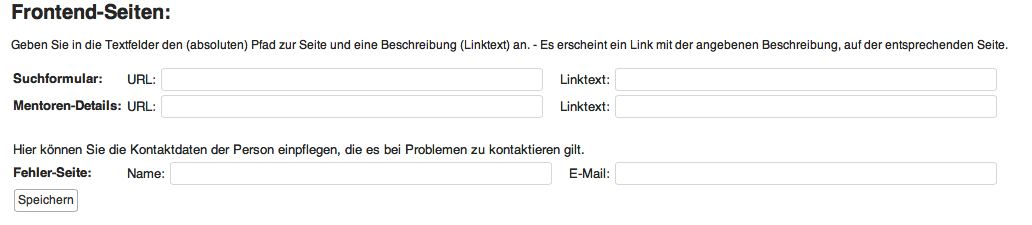
\includegraphics[angle={360}, scale=0.45]{pictures/form.png}
	    \caption{Beispielformular mittels PHP}
	    \label{img:BSPFORM}
	\end{center}
   \end{figure}
   \ \newline
Der Zweck dieses Formulars ist es, Einstellungen für das Plugin vorzunehmen. Dies geschieht in Form von Textfeldern, welche entsprechend ausgefüllt werden müssen.\newline
Erkennen lassen sich in Zeile 5 und Zeile 22 - 29 die POST-Methode. \newline
Nachdem die einzelnen Daten in die dafür vorgesehenen Felder eingetragen und der Speicher-Button aktiviert (\emph{ms\_options\_save}) wurde, wird in Zeile 22 die Funktion \emph{ms\_options\_update} aufgerufen. Der Zweck hinter dieser Funktion liegt darin, die Einstellungen für die Daten des geänderten Mentoren oder Mentees zu ändern.\newline
So würde ein Beispiel für eine Post-Methode in der Mentoren-Suche aussehen. Weitere Informationen zu dem Thema finden sich unter:
\begin{itemize}
	\item \url{http://www.selfphp.info/praxisbuch/index.php}
	\item \url{http://www.phpbox.de/php\_tutorials/formularversenden1.php}
\end{itemize}
\subsubsection{Beispiel für Wordpress-Formular}
Nachdem ein Beispiel mit der POST-Methode gezeigt und erläutert wurde, wird nun die Wordpress-Variante behandelt.\newline
Wie schon angesprochen, wird bei dieser Art die do\_action-Anweisung verwendet (vgl. \ref{wpform}). Diese ist beispielhaft in Listing \ref{BSPFORMINWP} dargestellt.
\lstset{language={PHP},caption={Beispiel Formular in Wordpress},label=BSPFORMINWP}
\lstset{
 morekeywords={function,do_action,global,\$exit_msg}
}
\begin{lstlisting}
function ms_row_new() {
	
	global $wpdb;
	global $title;
	echo "<h1>".$title."</h1>";
	
	echo "<div id=\"ms_row_new\">  
        <div class=\"register-form\">  
        <div class=\"title\">  ".
           "<h3>".__('Mentor eintragen','mentoren-suche')."</h3>
        </div>  
        <form
           //Formular

		  do_action('ms_insert_mentor');
			
		  echo " <input type=\"submit\" value=\"Eintragen\" id=\"register\" />  
		  
        </form>  
	</div>
</div>  ";

...
?>
\end{lstlisting}
Die in Listing \ref{BSPFORMINWP} dargestellte Funktion hat den Zweck, die Oberfläche für "Datensatz eintragen" funktional darzustellen. Dies ist in Abbildung \ref{img:BSPFORMWP} bildhaft dargestellt.
  \begin{figure}[htbp]
	\begin{center}
	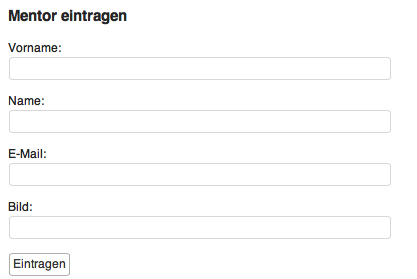
\includegraphics[angle={360}, scale=0.46]{pictures/formwp.png}
	    \caption{Beispielformular mittels do\_action}
	    \label{img:BSPFORMWP}
	\end{center}
   \end{figure}\ \newline
Was sich direkt erkennen lässt, sind die beiden Form-Tags in den Zeilen 12 und 19. Dazwischen befindet sich zum einen das Formular, zum anderen aber auch ein Button (\emph{Eintragen}) zum Bestätigen der Eingabe und ich Zeile 15 die \emph{do\_action}-Anweisung.\newline
Was hier nun passiert ist einfach zu erklären: Mittels der \emph{do\_action}-Anweisung wird die Action \emph{ms\_insert\_mentor} aufgerufen. Diese wiederum ruft in der Hauptdatei \emph{mentoren\_suche.php} die Action ms\_m\_data\_insert auf (siehe Listing \ref{AUACDDOACANW}).
\lstset{language={PHP},caption={Ausgeführte Action der do\_action-Anweisung},label=AUACDDOACANW}
\lstset{
 morekeywords={function,do_action,global,\$exit_msg}
}
\begin{lstlisting}
<?php
...
add_action('ms_insert_mentor','ms_m_data_insert');
...
<?
\end{lstlisting}
Diese wiederum ist dafür verantwortlich, nach dem Bestätigen des Submit-Buttons aus der Zeile 17 des Listing \ref{BSPFORMINWP}, die angegebenen Mentoren in die Mentorentabelle der Datenbank einzutragen.\newline
Vollständigerweise ist diese Funktion in Listing \ref{AUFGERACT} dargestellt und wird anschließend kurz erläutert.
\lstset{language={PHP},caption={Aufgerufene Funktion der Action},label=AUFGERACT}
\lstset{
 morekeywords={function,do_action,global,\$exit_msg}
}
\begin{lstlisting}
function ms_m_data_insert() {

	global $wpdb;

	if(isset($_POST['ms_m_name']) and isset($_POST['ms_m_vorname']) and isset($_POST['ms_m_email'])) {

	if(!empty($_POST['ms_m_name']) && !empty($_POST['ms_m_vorname']) && !empty($_POST['ms_m_email']))
	{		
	  $name = $_POST['ms_m_name']; 
	  $vorname = $_POST['ms_m_vorname']; 
	  $email = $_POST['ms_m_email'];
	  $bild = $_POST['ms_m_bild'];
	
	$rows_affected = $wpdb->insert(MENTOR_TABLE, array( 'mentoren_name' => $name, 'mentoren_vorname' => $vorname, 'mentoren_email' => $email, 'mentoren_bild' => $bild, ) );
	
	} else {
		... //Fehlermeldung
	}

	}
}
\end{lstlisting}
Insgesamt besteht die Funktion aus zwei IF-Abfragen. Dabei soll die erste (Zeile 5) laut PHP.net\footcitetint[Vgl.][]{THPHPISSET13} prüfen, ob eine Variable existiert und nicht NULL ist. Falls dies der Fall sein sollte, wird die nächste IF-Abfrage (Zeile 7) prüfen, ob die Inhalte des Formulars befüllt sind - spricht nicht leer sind. Anschließend wird, wenn die Bedingung erfüllt ist, die entsprechenden Daten des Formulars in Variablen übertragen (Zeile 9 - 12) und in Zeile 14 dann in die Datenbank eingetragen. Bei dem nicht Zutreffen einer Bedingung wird automatisch die Funktion beendet.\newline
Nachdem die beiden Versionen von Formularen vorgestellt wurden, kann sich formulieren lassen, dass die PHP-Version zwar um einiges kürzer ist als die von Wordpress. Beide sind allerdings funktional gesehen gleichwertig zu betrachten.\newline
Damit soll das Kapitel Formulare beendet sein und dem nächsten Kapitel zugewandt. Dieses handelt von der Internationalisierung und Lokalisation von Wordpress-Plugins.
\newpage
%%
%%%%********************************************************************************
\section{Internationalisierung und Lokalisierung}\label{interundlok}
In diesem Kapitel wird die Internationalisierung und Lokalisierung von Wordpressplugins beschrieben und anhand von Beispielen erläutert. Dazu wird erst eine Einleitung in Abschnitt \ref{allgemeinesil} gegeben, die die Begrifflichkeiten und den Sinn dieser Technik vorstellt. Im Abschnitt \ref{sub:lokalisierung} wird beschrieben, wie die Lokalisierung (innerhalb des Programmcodes) erfolgt. Danach erfolgt die Beschreibung im Abschnitt \ref{sub:letd}, wie eine Textdomäne geladen werden kann. Der Abschnitt \ref{sub:adue} beschreibt, wie die eigentlichen Texte (Zeichenketten) übersetzt werden. Abschließend wird im Abschnitt\ref{sub:confdwpspr} kurz gezeigt, wie die Sprache des Wordpress-Systems konfiguriert werden kann.
\subsection{Einführung}\label{allgemeinesil}
Bei der Internationalisierung und Lokalisierung handelt es sich um ein allgemeines Konzept in der Programmierung. \newline
Nach Shirah\footcitetint[Vgl.][]{JSS02} handelt es sich bei der Internationalisierung (engl. internationalization)  um einen ,,Prozess der Erstellung einer Software für den Einsatz im multinationalen Kontext'' (eigene Übersetzung). Neben der Unterstützung von unterschiedlichen Sprachen, ist die Software auch in der Lage, mit unterschiedlichen Datums-, Zeit-, Währungsformaten umzugehen. Dabei ist bedeutsam, dass dies ohne Eingriff in den Programmcode erfolgt. Unter Praktikern ist für den Begriff ,,Internationalization'' die Abkürzung ,,I18N'' (steht für: die 18 Buchstaben zwischen dem ,,I'' und dem ,,N'' des Wortes ,,Internationalization'') gebräuchlich.\newline
Die Lokalisierung (abgekürzt häufig: ,,L10N'', nach ähnlicher Semantik wie bei dem Begriff ,,Internationalisierung'') ist als Bestandteil der Internationalisierung zu verstehen. Darunter ist die Vorbereitung des Programms für den Umgang mit unterschiedlichen Sprachen, Kulturen sowie Ländern gemeint.  Shirah beschreibt sehr anschaulich, wie die Lokalisierung praktisch zu verstehen ist. Zur Verhinderung einer Verfälschung der Aussage, wird  die entsprechende, englische Passage aus dem Originaltext zitiert: „Usually, though, true localization is archived by core code that accesses locale, location, political, or other specific components an modules, along with translating text as appropriate for the audience“.\newline
Die Lokalisierung kann demnach als eine Aktivität innerhalb der Internationalisierung verstanden werden: Hier geht es um die Übersetzung der vorbereitenden Daten in einem Nutzungskontext. Ein Benutzer greift mittels eines Browsers auf eine Seite zu und die Wordpress-Umgebung verwendet direkt die richtige Sprache für die Oberflächenelemente. Dabei ist  zu beachten, dass die Lokalisierung immer lokal stattfindet. Dies bedeutet, dass die Spracheinstellungen in der Hauptkonfiguration von Wordpress (wp-config.php) eine wichtige Rolle spielen: Je nach konfigurierter Sprache, werden die entsprechenden Sprachdateien verwendet (sofern diese vorhanden sind). Bei dieser Art von Übersetzungen sind lediglich die Oberflächenelemente betroffen. Eine Übersetzung der Inhalte der Webseiten/Plugins (Einstellungsdaten, Beiträge, Seiten) erfolgt hierüber nicht. Dies muss über entsprechende Plugins geschehen, die es ermöglichen Inhalte für beispielsweise 
'Artikel/Seiten in mehreren Sprachen abzulegen. Dazu stehen beispielsweise folgende Plugins zur Verfügung: \emph{gTranslate} (Download (\url{http://wordpress.org/extend/plugins/qtranslate/screenshots/})  oder \emph{WPML} (Download unter: \url{http://wpml.org}).\newline
Wordpress nutzt im Speziellen das gettext-Framework (PHP), dass zur Internationalisierung einer Anwendung konzipiert ist\footcitetint[Vgl.][]{TPGGT}. Weitere Informationen zum Framework unter: \url{http://www.php.net/manual/de/book.gettext.php}.
\subsection{Lokalisierung}\label{sub:lokalisierung}
In diesem Abschnitt wird gezeigt, wie in Wordpress-Programmcode die Lokalisierung vorgenommen wird. Hierbei wird sich lediglich auf die Elemente der Oberfläche (Beschriftungen) beschränkt (vgl. Abschnitt \ref{allgemeinesil}).\newline
Zur Lokalisierung werden spezielle Funktionen an die Stellen des Quellcode hinzugefügt, die ansonsten Zeichenketten (Beschriftungen von Oberflächenelementen, Fehlermeldungen) in eine Sprache enthalten würden. \newline Dabei sind folgende Funktionen zu nennen\footcitetint[Vgl.][Seite 238]{BB11}:
\begin{enumerate}
	\item \_e(\$message,\$domain)
	\begin{itemize}
		\item Diese Funktion sucht das „Lokalisierungsmodul“ (eigene Übersetzung) nach einer Übersetzung, für die in der Variablen \$message gespeicherten Zeichenkette. Wird eine entsprechende Übersetzung gefunden, wird diese auf dem Bildschirm ausgegeben (e steht für die echo-Anweisung). Sollte keine Übersetzung vorhanden sein bzw. gefunden werden, wird der Inhalt in der Variablen \$message direkt ausgegeben. Der Parameter \$domain steht für die Angabe einer Textdomäne, in der die Zeichenkette hier verwendet werden soll. Das Konzept der Textdomäne wird im Abschnitt \ref{sub:letd} thematisiert.\newline 
		Im Listing \ref{CBSPVERWE} ist ein Beispiel für die Verwendung der oben beschriebenen Funktion zu erkennen. Dort wird lediglich ein Hinweis lokalisiert, der sich auf dem CSV-Import des Mentoren-Suche-Plugins bezieht.
\lstset{language={PHP},caption={Beispiel für die Verwendung von \_e()},label=CBSPVERWE}
\lstset{
 morekeywords={function,do_action,global,\$exit_msg,\$wpdb}
}
\begin{lstlisting}
<?php 
...
_e('Bitte eine Datei ausw&auml;hlen die Mentee Daten beinhaltet.','mentoren-suche');
...
?> 
\end{lstlisting}		
				
	\end{itemize}
	\item \_ \_(\$message,domain)
	\begin{itemize}
	\item Diese Funktion übernimmt dieselbe Aufgabe wie \_e(). Auch gelten dieselben Erläuterungen zum Parameter \$domain. Der Unterschied ist, dass der (übersetzte) Text nicht ausgegeben wird, sondern die Zeichenkette (string) zurückgegeben wird, sodass diese in einer return-Anweisung verwendet werden kann oder in einer Zeichenkette integriert werden kann.\newline
	Im Listing \ref{CBSPVERWEE} ist ein Beispiel für die Verwendung der Funktion \_ \_() zu erkennen. Hier wird 
eine formatierte Fehlermeldung lokalisiert.
\lstset{language={PHP},caption={Beispiel für die Verwendung von \_ \_()},label=CBSPVERWEE}
\lstset{
 morekeywords={function,do_action,global,\$exit_msg,\$wpdb}
}
\begin{lstlisting}
<?php 
...
echo "<h3 class=\"ms_error_message\">".__('Bitte alle Pflichtfelder ausf&uumlllen!','mentoren-suche')."</h3>";	
...
?> 
\end{lstlisting}		
\end{itemize}	 
\end{enumerate}   
Nach der Darstellung der beiden, wichtigsten Lokalisierungsfunktionen, sollen auch einige Hinweise zur praktischen Verwendung gegeben werden. Dazu liefern Bondari/Griffiths\footcitetint[Vgl.][Seite 240ff.]{BB11} einige „Best Practice“-Empfehlungen. Für die Entwicklung des Beispiel-Plugins „Mentoren-Suche“ waren drei Empfehlungen bedeutsam. Diese sollen nun kurz beschrieben werden:
\begin{enumerate}
	\item Es sollen Leerzeichen am Anfang und am Ende der zu übersetzenden Zeichenkette vermieden werden. Dies kann überraschende Auswirkungen auf die Übersetzung der Zeichenkette haben. Denn aus der Programmierung ist bekannt, dass die Zeichenkette „Hallo Welt“ ungleich „ Hallo Welt“ ist.
	\item Außerdem soll HTML und URLs in einer zu übersetzenden Zeichenkette vermieden werden. Als ein Grund kann sich vorgestellt werden, dass derjenige, der die Übersetzungen vornimmt (muss nicht unbedingt ein Programmierer sein, vgl. Abschnitt \ref{sub:adue}) auch daran denken müsste, die HTML-Befehle und URLs in der Übersetzung korrekt zu integrieren. \newline Ein Beispiel für eine Fehlermeldung, die formatiert mit HTML (und CSS) wird, zeigt eine mögliche Realisierung (vgl. Listing \ref{CBSPVERWEE}). Es erfolgt eine Konkatenation mehrerer Zeichenketten. Die geöffneten und schließenden Tags sind jeweils eine Teil-Zeichenkette, die mit der zu übersetzenden Zeichenketten verknüpft wird. 
\item Ferner sollen keine Variablen in der zu übersetzenden Phrase enthalten sein. Hierfür kann derselbe Grund angegeben werden, wie unter Punkt 2. Der Übersetzer müsste auch die Variablen wieder korrekt in die Übersetzung integrieren. Erfolgt dies nicht korrekt, könnte das Programm unsinnige Meldungen ausgeben.\newline
Die Einbettung der Variablen in einer zu übersetzenden Phrase kann über Platzhaltern in der Zeichenkette geschehen. Dies kann mit der sprintf()-Funktion realisiert werden, die eine formatierte Zeichenkette zurückliefert.\footcitetint[Vgl.][]{TPGGT}\newline
Das folgende Beispiel (vgl. Listing \ref{CBSPEINBSP}) demonstriert die Verwendung dieser Funktion im Lokalisierungskontext.
\lstset{language={PHP},caption={Beispiel für die korrekte Einbettung von Variablen mit der sprintf()-Funktion},label=CBSPEINBSP}
\lstset{
 morekeywords={function,do_action,global,\$exit_msg,\$wpdb}
}
\begin{lstlisting}
<?php 
...
echo "..."
sprintf( __('Mentor %s wurde mit seinem Nachnamen angelegt, bitte Mentoren Stammdaten vervollst&auml;ndigen','mentoren-suche'), utf8_encode($teile[0]))	
...
?> 
\end{lstlisting}	
Das aus dem „Mentoren-Suche“-Plugin entnommene Code-Fragment (vgl. Listing \ref{CBSPEINBSP}) wurde gekürzt (angedeutet mit ...). Denn es sollen hier nur die für die Erklärung benötigten Elemente enthalten sein.
Es ist zu erkennen, dass innerhalb von sprintf() die Lokalsierungsfunktion \_ \_() verwendet wird. In dieser Funktion befindet sich die zu übersetzenden Zeichenkette. Dort befindet sich für den Namen des Mentors der Platzhalter \%s. Der entsprechende Wert wird vom Ausdruck  zurückgeliefert, der nach dem (ersten) Komma angegeben ist: utf8\_encode(\$teile[0]).
Somit lässt sich sehr einfach, den Einsatz von Variablen in Zeichenketten vermeiden.\end{enumerate}
Abschließend soll auf die Online-Ressource verwiesen werden, die weitere Hinweise zur  Lokalisierung bietet.: \url{http://codex.wordpress.org/I18n\_for\_WordPress\_Developers}.
Im nächsten Abschnitt \ref{sub:letd} wird das Laden einer Textdomäne behandelt. 
\subsection{Laden einer Textdomäne}\label{sub:letd}
In diesem Abschnitt soll das Konzept der „Textdomäne“ beschrieben werden und wie solch eine zur Laufzeit geladen werden kann.
In der (natürlichen) Sprache sind Wörter mehrdeutig und damit vom Kontext abhängig.
Damit Wörter für einen geltenden Kontext übersetzt werden können, gibt es das Konzept der Textdomäne. Ein Beispiel soll die Erklärungen verdeutlichen: Das Wort \emph{football} gibt es zwar im britischen und amerikanischen Englisch, wird allerdings je nach Land anders interpretiert. Die Textdomäne hilft die Bedeutung gleicher Wörter zu unterscheiden\footcitetint[Vgl.][Seite 239]{BB11}.\newline
Im Folgenden soll beschrieben werden, wie eine Textdomäne im Quellcode geladen wird. Dazu soll anhand von Listings \ref{CLDTXD} (aus dem Plugin „Mentoren-Suche“) die Funktionsweise erläutert werden.
\lstset{language={PHP},caption={Laden einer Textdomäne},label=CLDTXD}
\lstset{
 morekeywords={function,do_action,global,\$exit_msg,\$wpdb}
}
\begin{lstlisting}
<?php 
...
add_action('init','ms_load_translation_file'); 
...
...
function ms_load_translation_file(){
  $plugin_path =   
        plugin_basename(dirname(__FILE__).'/lang');
  load_plugin_textdomain('mentoren-suche',false, 
                         $plugin_path); 
}
...
?> 
\end{lstlisting}	
Die erste relevante Anweisung (vgl. Listing \ref{CLDTXD}) fügt der Wordpress-Engine ein Ereignis hinzu.
Mit dem (vordefinierten) Ereignis init wird nachdem Laden von Wordpress die hier angegebene Funktion ms\_load\_translation\_file aufgerufen. In dieser befindet sich der eigentliche Code für die Registrierung der Textdomäne:
Die Funktion plugin\_basename ermittelt den Pluginname. Das macht die Funktion dadurch, indem sie vom übergebenen Dateinamen/Verzeichnisnamen den Pluginnamen extrahiert\footcitetint[Vgl.][]{MMTFRPL13}.\newline
Dazu ist es erforderlich, dass der gesamte Pfad zur Plugin-Datei übergeben wird. Dies geschieht mittels der PHP-Funktion dirname, die als Parameter hier die vordefinierte PHP-Konstante \_\_FILE\_\_ übergeben bekommt. Die PHP-Konstante \_\_FILE\_\_ enthält den absoluten Pfad zur Datei, in der diese Konstante aufgerufen wird\footcitetint[Vgl.][]{TPGMK}.\newline
Die Funktion dirname gibt,  auf Basis des übergebenen Pfads, das übergeordnete Verzeichnis zurück\footcitetint[Vgl.][]{TPGDN}.
Per Konkatenation wird das dynamisch ermittelte Verzeichnis des Plugins mit dem Verzeichnisnamen ,,lang'' verknüpft. In diesem Verzeichnis sollen die Sprachdateien werden die Sprachdateien (vgl. Abschnitt \ref{sub:adue}) für das Plugin abgelegt. Der Name hätte beispielsweise auch anders gewählt werden können: ,,language''. \newline
Zusammenfassend erledigt die erste Zeile folgendes: es wird mehr oder weniger dynamisch das Verzeichnis festgelegt/bestimmt, in dem die relevanten Sprachdateien liegen. Diese Information wird in die Variable \$plugin\_path gespeichert.
Die Funktion load\_plugin\_textdomain ist für das Laden der Textdomäne zuständig. Zur eindeutigen Identifikation der Textdomäne wird die Domainbezeichnung (erster Parameter) angegeben (hier: mentoren-suche). Der Domainnamen darf einzig aus alphabetischen Zeichen, Bindestrichen und Unterstrichen bestehen. Bondari/Griffiths empfehlen den Pluginnamen zu verwenden\footcitetgedr[Vgl.][Seite 240]{BB11}.\newline
Die Textdomäne wird als zweiter Parameter der Lokalisierungsfunktionen \_e() und \_\_() übergeben (vgl. Abschnitt \ref{sub:lokalisierung}).\newline
Der zweite Parameter ist veraltet (deprecated) und soll nicht mehr verwendet werden. Dieser wird standardmäßig auf false gesetzt und wird hier nicht weiter betrachtet. Als dritten Parameter wird  die in der Variablen \$plugin\_path  gespeicherten Information (Pfad, in der die Sprachdateien abgelegt werden) übergeben.\newline
In diesem Abschnitt wurde das Konzept der Textdomäne vorgestellt, dass zur eindeutigen Verwendung von übersetzenden Wörtern/Phrasen eingesetzt wird. Es wurde vorgestellt, wie solch eine Textdomäne im Quellcode registriert wird. Im nächsten Abschnitt wird beschrieben, wie die eigentlichen Sprachdateien (mit den Übersetzungen) erzeugt werden.
\subsection{Anlegen der Übersetzung}\label{sub:adue}
In diesem Abschnitt wird vorgestellt, wie die eigentlichen Übersetzungen entstehen. Dazu ist es erforderlich, ein Programm zu nutzen, um die lokalisierten Phrasen/Begriffe im Quellcode, in die gewünschte Sprache zu übersetzen und in spezielle Sprachdateien abzulegen. Das hier eingesetzte Programm heißt „Poedit“ (Download unter: \url{http://www.poedit.net} ). Neben diesem Programm, existieren weitere für diesen Zweck. Eine Liste findet sich unter: \url{http://codex.wordpress.org/Translating\_WordPress\#Translation\_Tools}.
\newline
Im Folgenden soll die Erstellung von Sprachdateien mittels  „Poedit“ geschildert werden\footcitetgedr[Vgl.][Seite 245 - 249]{BB11}:
\begin{enumerate}
	\item Starten des Tools „Poedit“
	\item „Datei“ \textgreater „Neuer Katalog“. Es erscheint der Dialog „Katalogoptionen“. Es müssen alle drei Reiter abgearbeitet werden, bevor auf OK geklickt wird. Dies bitte unbedingt beachten!
	\begin{itemize}
\item \emph{Reiter „Projektinfo“}: Hier werden grundlegende Informationen zum Projekt angegeben. Zum Beispiel: Projektname und -version, Sprache, Land, Zeichensatz, Übersetzerteams. In diesem Beispiel soll die Übersetzung in die englische Sprache (US) erfolgen (vgl. Abbildung \ref{img:KRP}).
   \begin{figure}[htbp]
	\begin{center}
	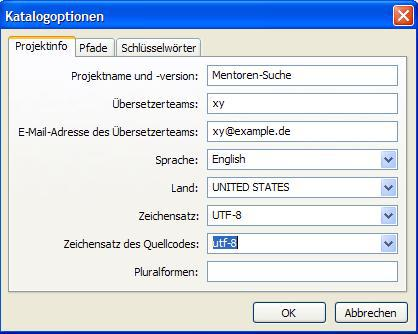
\includegraphics[angle={360}, scale=0.45]{pictures/lok1.jpg}
	    \caption{Katalogoptionen - Reiter ,,Projektinfo''}
	    \label{img:KRP}
	\end{center}
   \end{figure}
   \item \emph{Reiter „Pfade“}: Hier wird der relative Pfad, ausgehend vom Plugin-Sprachverzeichnis zum  Plugin-Basisverzeichnis angegeben. Zur Erinnerung: in diesem Beispiel nannte sich das Sprachverzeichnis „lang“, dass direkt im Plugin-Basisverzeichnis liegt. 
   \item Als Pfad muss hier also eingegeben werden: „..“ (2 Punkte für das Wechseln in eine Verzeichnisebene nach oben) (vgl. Abbildung \ref{img:KRPF}).
   \begin{figure}[htbp]
	\begin{center}
	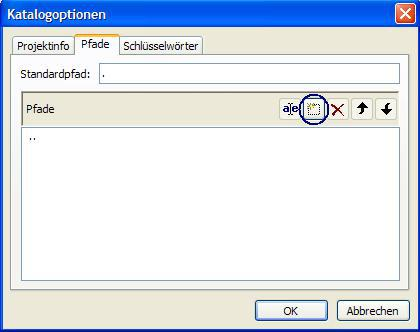
\includegraphics[angle={360}, scale=0.45]{pictures/lok2.jpg}
	    \caption{Katalogoptionen - Reiter ,,Pfade''}
	    \label{img:KRPF}
	\end{center}
   \end{figure}
\newpage
\item \emph{Reiter ''Schlüsselwörter''}: Hier werden die Funktionsnamen der Liste hinzugefügt, an denen die zu übersetzenden Begriffe/Phrasen erkannt werden. Das wären hier in diesem Fall: \_ \_ und \_e.  Alle bereits vorhandenen Funktionsnamen müssen aus der Liste entfernt werden (vgl. Abbildung \ref{img:KRSCH}).
   \begin{figure}[htbp]
	\begin{center}
	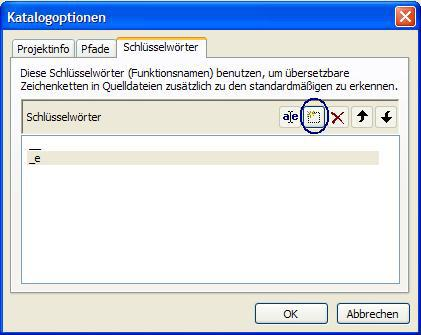
\includegraphics[angle={360}, scale=0.45]{pictures/lok3.jpg}
	    \caption{Katalogoptionen - Reiter ,,Schlüsselwörter''}
	    \label{img:KRSCH}
	\end{center}
   \end{figure}
   \item Nach Berücksichtigung aller Reiter, darf nun die Schaltfläche ''OK'' angeklickt werden. Es erscheint der Dialog ,,Speichern unter''. Die Datei sollte den Namen des Plugin-Ordners (hier: mentoren-suche) im  .pot-Format – innerhalb des Sprachverzeichnisses - abgespeichert werden. Also: mentoren-suche.pot (Anmerkung: Die \gls{POT}-Datei enthält alle Übersetzungen). Anschließend den Speichervorgang ausführen, indem die Schaltfläche ,,Speichern'' betätigt wird (vgl. Abbildung \ref{img:DSU}).
      \begin{figure}[htbp]
	\begin{center}
	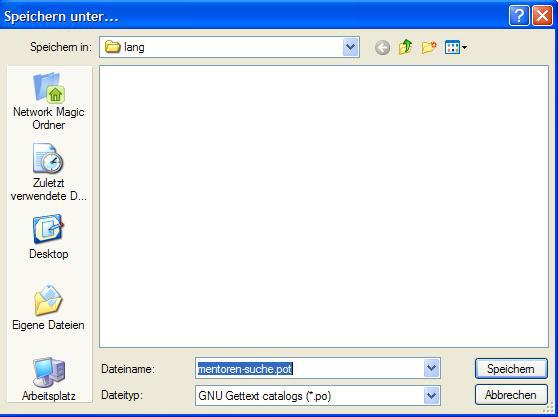
\includegraphics[angle={360}, scale=0.45]{pictures/lok4.jpg}
	    \caption{Katalogoptionen - Dialog ''Speichern unter''}
	    \label{img:DSU}
	\end{center}
   \end{figure}
   \item Nun werden alle Zeichenketten aus dem Quellcode herausgefiltert. Dazu erscheint die in der Abbildung  \ref{img:KMEUEAK} dargestellte Meldung.
     \begin{figure}[htbp]
	\begin{center}
	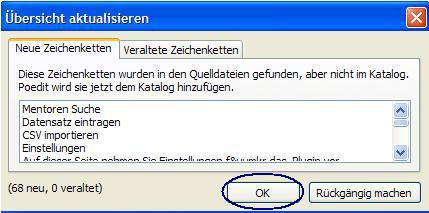
\includegraphics[angle={360}, scale=0.61]{pictures/lok5.jpg}
	    \caption{Katalogoptionen - Meldung ''Übersicht aktualisieren''}
	    \label{img:KMEUEAK}
	\end{center}
   \end{figure}   
   \newpage
   \item Nachdem Betätigen der Schaltfläche ''OK'', erscheinen alle zu übersetzenden Zeichenketten in der Oberfläche von ''Poedit'' (vgl. Abbildung \ref{img:POUEERS}).
Nun erfolgt die Übersetzung wie folgt: es wird sukzessive jede Zeichenkette vom Anwender (''Übersetzer'') angeklickt. Daraufhin erscheint im ersten unteren Textfeld die aktuelle, ausgewählte Originalzeichenkette. Im darunter liegenden Textfeld wird die entsprechende Übersetzung eingegeben. Danach wird auf das Icon ''Katalog speichern'' angeklickt. Nun ist die nächste Zeichenkette zu übersetzen. Die übersetzten Zeichenketten werden nach unten angehängt. Dies erfolgt gewöhnlich solange, bis alle Zeichenketten übersetzt sind.
     \begin{figure}[htbp]
	\begin{center}
	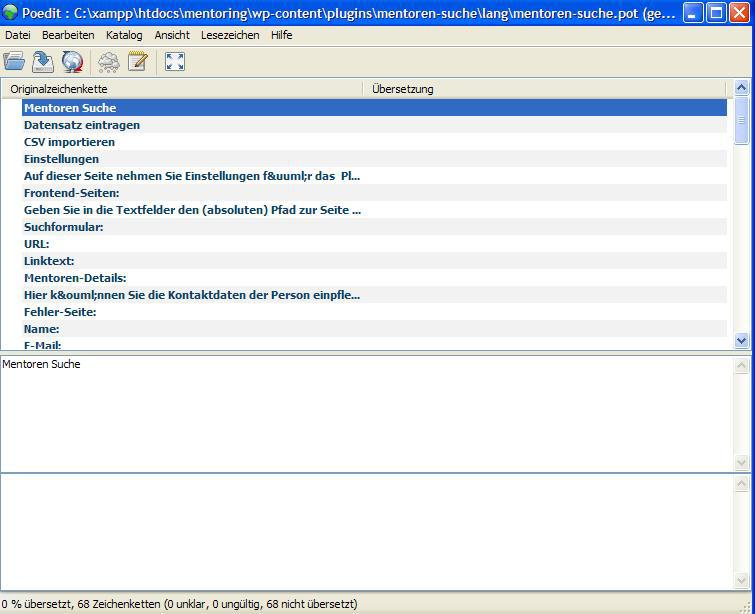
\includegraphics[angle={360}, scale=0.45]{pictures/lok6.jpg}
	    \caption{Poedit - Übersetzungen erstellen}
	    \label{img:POUEERS}
	\end{center}
   \end{figure} 
   \item Sind alle Zeichenketten übersetzt, muss eine Kopie der POT-Datei als PO-Datei
abgespeichert werden. Dies geschieht über ''Datei''  ''Speichern unter''.
Der Dateiname hat dabei folgende Konvention: \emph{pluginname-sprachcode\_Landcode.po}.
\begin{enumerate}
\item Der \emph{Sprachcode} entspricht dem Code nach ISO 639-1: siehe beispielsweise \url{http://en.wikipedia.org/wiki/List\_of\_ISO\_639-1\_codes}.
\item Der \emph{Ländercode} entspricht dem Code nach ISO 3166-1: siehe beispielsweise
\url{http://en.wikipedia.org/wiki/ISO\_3166-1}.
\end{enumerate}
Für die in diesem Beispiel englische Übersetzung (Land: USA), entsteht folgender Dateiname: \emph{mentoren-suche-en\_US.po}. 
\end{itemize}
\end{enumerate}
Damit ist der Übersetzungsprozess abgeschlossen. Es ist darauf hinzuweisen, dass neben den .po- und .pot-Dateien auch eine .mo-Datei angelegt wird. Dabei handelt es sich um eine binäre Version der .po-Datei. Diese ist nicht menschenlesbar.\footcitetgedr[Vgl.][Seite 249]{BB11}\newline
Der Prozess der Aktualisierung von bereits bestehenden Sprachdateien, soll hier nicht betrachtet werden, da dies den Rahmen dieses Tutorials sprengen würde. Denn dieser Vorgang wurde für die Entwicklung des Plugins ''Mentoren-Suche'' bisher nicht benötigt. Stattdessen wird auf Literatur Bondari/Griffiths\footcitetgedr[Vgl.][Seite 251]{BB11} verwiesen.\newline
Damit das Ergebnis der Übersetzung sichtbar ist, muss Wordpress auf die entsprechende Sprache eingestellt sein. Dies wird im nächsten Abschnitt \ref{sub:confdwpspr} beschrieben.
\subsection{Konfiguration der Wordpress-Sprache}\label{sub:confdwpspr}
Im Kapitel \ref{allgemeinesil} wurde bereits erwähnt, dass die Sprachkonfiguration von Wordpress zentral in der Konfigurationsdatei wp-config.php geschieht. In diesem Abschnitt soll vorgestellt werden, wie diese Einstellung vorgenommen wird.\newline
Die entscheidende Code-Zeile in der wp-config.php-Datei ist folgende (vgl. Listing \ref{WPLANG}).
\lstset{language={PHP},caption={wp-config.php – Die in PHP definierte Konstante WPLANG},label=WPLANG}
\lstset{
 morekeywords={function,do_action,global,\$exit_msg,\$wpdb}
}
\begin{lstlisting}
<?php 
...
define('WPLANG', 'de_DE');
...
?> 
\end{lstlisting}	
In Listing \ref{WPLANG} ist die definierte Konstante WPLANG für die zentrale Spracheinstellung der Wordpress-Oberfläche zu sehen. Der Wert der Konstante (hier: de\_DE) entspricht demselben Schema (Sprachcode/Ländercode nach ISO), wie es im Abschnitt \ref{sub:adue} beschrieben wird.\newline
Dabei ist zu beachten, dass sowohl für die jeweiligen Plugins die entsprechende Sprachdateien mitgeliefert werden müssen als auch im Wordpress-Verzeichnis wp-content/languages die Sprachdateien vorhanden sind. Ansonsten würde die Spracheinstellung keine oder nur unbefriedigende Auswirkungen haben.\newline
Zum Abschluss soll gezeigt werden, wie die Übersetzung anhand des Beispiel-Plugins ''Mentoren-Suche'' aussieht. Dazu muss in der wp-config.php (wie in diesem Abschnitt beschrieben) die Sprache englisch (für das Land USA) eingestellt werden. Der Wert für die Konstante lautet wie folgt: en\_US (kann von den Sprachdateien abgeschaut werden. Zum Beispiel:  mentoren-suche-en\_US.po).\newline
Das Ergebnis der Übersetzung wird im Folgenden für die Suchmaske im Frontend demonstriert (vgl. Abbildung \ref{img:DSDE} für die deutsche Spracheinstellung [Standard] und vgl. Abbildung \ref{img:ESEIN} für die englische Spracheinstellung).
   \begin{figure}[htbp]
	\begin{center}
		
\includegraphics[angle={360}, scale=0.61]{pictures/de1.jpg}
	    \caption{Deutsche Spracheinstellung (de\_DE) [Standard]}
	    \label{img:DSDE}
	    	\end{center}
	    	\begin{center}
		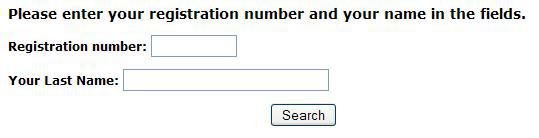
\includegraphics[angle={360}, scale=0.61]{pictures/de2.jpg}
	    \caption{Englische Spracheinstellung (en\_US)}
	    \label{img:ESEIN}
	    	\end{center}
   \end{figure} 
\ \newline
\newpage
\newpage
%%
%%%%********************************************************************************
 \section{Pluginverwendung in Wordpress}\label{PLASDA}
Nachdem die Programmierung des Plugins soweit abgeschlossen ist und die fundamentalen Kenntnisse erklärt und entsprechende Funktionen erläutert wurden, widmet sich dieses Kapitel mit der Installation und Deinstallation des Plugins. \newline
Dabei sollte beachtet werden, dass auch hier aus Programmier- und nicht primär aus Anwendersicht erläutert und erklärt wird.
Zuvor soll allerdings eine kleine Begriffsbestimmung für dieses Kapitel geschehen.
\subsection{Unterscheidung der Installationstypen}
Wie schon bereits angedeutet, soll an dieser Stelle zuerst einmal die unterschiedlichen Typen von Installation und Deinstallation eines Wordpress-Plugins angesprochen werden. Allgemein wird dabei in drei verschiedenen Zuständen unterschieden. Diese werden nun dargestellt, um anschließend mit den einzelnen Installations- und Deinstallationsroutinen fortzufahren.\newline
Laut Williams/Richard/Tadlock\footcitetgedr[Vgl.][Seite 20 - 22]{BWPWP11} sind die drei Zustände folgendermaßen beschrieben:
\begin{enumerate}
	\item \textbf{Aktivierungfunktionen}
	\begin{itemize}
		\item Diese Art von Funktionen werden dann aufgerufen, wenn ein Benutzer mit entsprechenden Administrationsrechten dieses Plugin aktiviert. 
\end{itemize}		
	\item \textbf{Deaktivierungsfunktionen}
	\begin{itemize}
		\item Auch diese Funktion verhält sich ähnlich wie die Aktivierungsfunktionen, mit dem kleinen Unterschied, dass diese erst dann ausgeführt werden, wenn der Administrator das zuvor aktivierte Plugin deaktiviert.
	\end{itemize}
	\item \textbf{Deinstallationsfunktionen}
	\begin{itemize}
		\item Nachdem ein Plugin deaktiviert wurde, kann es auch deinstalliert werden. Dabei werden alle Einstellungen sowie das Plugin selbst gelöscht. Eine solche Funktion sollte in jedem Plugin vorhanden sein, um dem User einen angenehmen Weg zur Deinstallation zu bieten und das Plugin professionell abzurunden.
	\end{itemize}
\end{enumerate}
Soweit an dieser Stelle zu den einzelnen Funktionsunterscheidungen. Das nächste Kapitel beschäftigt sich mit den einzelnen Routinen.
\subsection{Installation}
Ein jedes abgeschlossene Plugin sollte bei entsprechender Funktionalität und Entwicklungsstadium irgendwann installiert werden. Genau dies wird in diesem Unterkapitel angesprochenen.\newline
Allgemein lässt sich formulieren, dass ein Plugin über die Administratoroberfläche unter dem Pfad \emph{Plugins/Installieren} installiert werden kann.\newline
Was dabei im Hintergrund passiert, das heißt genauer: Was aus Entwicklerperspektive passiert, ist im Unterkapitel \ref{insrout} weiter beschrieben. 
\subsubsection{Intallationsroutinen}\label{insrout}
Sogenannte Installationsroutinen werden bei der Aktivierung (vgl. Abschnitt \ref{aktvfunk}), Deaktivierung (vgl. Abschnitt \ref{Deaktivieren}) und Löschen (vgl. Abschnitt \ref{Deinstallieren}) des Plugins angestoßen - also automatisch ausgeführt.\newline
Der Vorteil bei solchen Installationsroutinen liegt darin, bestimmte Standardeinstellungen des Plugins zu setzen. Die hier angesprochenen Funktionen sind Fundamental und lassen sich für alle Plugins einsetzen.\footcitetgedr[Vgl.][Seite 18]{BWPWP11}\newline
Um die genaueren Eigenschaften einer solchen Aktivierungsfunktion kennen zu lernen, wird diese nun in Abschnitt \ref{aktvfunk} besprochen.
\paragraph{Aktivieren}\label{aktvfunk}\ \newline
Bei der Aktivierung werden einzelne Definitionen, Action, Options und Funktionen ausgeführt. Beispielweise können somit die initialen Tabellen oder bestimmte Funktionen ausgeführt werden. An dieser Stelle sollen solche in dem Plugin verwendeten Objekte vorgestellt werden.
\subparagraph{Plugin-Activation-Funktion}\ \newline
Diese Funktion dient dazu, direkt bei der Aktivierung des Benutzers ausgeführt zu werden. Hiermit lassen sich einige Standardeinstellungen festlegen. Natürlich lassen sich beispielsweise auch Versionsprüfungen oder verschiedenen Datenbanktabellen anlegen.\newline
Dies soll an folgenden Listing \ref{BSPACTHOO} weiter erklärt werden:
\lstset{language={PHP},caption={Beispiel für einen Activation-Hook},label=BSPACTHOO}
\lstset{
 morekeywords={function,do_action,global,\$exit_msg,\$wpdb}
}
\begin{lstlisting}
<?php 
...
register_activation_hook( $file, $function ); 
...
?> 
\end{lstlisting}
Wie dargestellt, sieht syntaktisch so eine Funktion aus, welche bei aktivieren des Plugins ausgeführt wird. Dabei sind die folgenden Parameter zu beachten\footcitetgedr[Vgl.][Seite 18]{BWPWP11}:
\begin{enumerate}
	\item \textbf{\$file}
	\begin{itemize}
		\item Hierbei handelt es sich um einen String-Parameter, welcher für den Pfad zu der Hauptdatei des Plugins bestimmt ist. Dies könnte also beispielsweise die Datei \emph{mentoren\_suche.php} sein.
	\end{itemize}
	\item \textbf{\$function}
	\begin{itemize}
		\item Diese hier angegebene Funktion wird dann aufgerufen, wenn die Aktivierung des Plugins stattfindet.
	\end{itemize}
\end{enumerate}
Ein Beispiel kann diese Definition veranschaulichen (siehe Listing \ref{BSPACTHOO})
\lstset{language={PHP},caption={Beispiel für einen Activation-Hook},label=BSPACTHOO}
\lstset{
 morekeywords={function,do_action,global,\$exit_msg,\$wpdb}
}
\begin{lstlisting}
<?php 
...
register_activation_hook( __FILE__, 'boj_myplugin_install' );
function INSTALL() { //do cool activation stuff
}
...
?> 
\end{lstlisting}
Wenn also die Aktivierung des Plugins erfolgt, wird die Funktion INSTALL() aufgerufen. Allerdings soll es hier ein Anliegen sein, die PHP-Konstante \emph{\_\_FILE\_\_} zu erläutern.\newline
Wie bereits in der Definition erwähnt, soll der erste Parameter den Pfad zur Hauptdatei des Plugins darstellen. Mittels die FILE-Konstante von PHP, wird automatisch der absolute Pfad des Plugins zu der Datei ermittelt, welche die Funktion aufruft.\footcitetgedr[Vgl.][Seite 18]{BWPWP11}\newline
Nachdem die grundlegende Aktivierungsfunktion besprochen wurde, sollen nun auch ein paar Actions besprochen werden, welche für die Aktivierung des Plugins interessant sind.
\subparagraph{Das Event init}\ \newline
Das erste Event, welches hier besprochen wird, ist das init-Event von Wordpress.\newline
Wie in Listing \label{MIVERSWP} dargestellt, wird mittels des Hooks \emph{Action} (siehe Kapitel \ref{sub_acvsfs}) und dem Event \emph{Init} die Funktion \emph{MS\_MIN\_WORDPRESS\_VERSION} aufgerufen.
\lstset{language={PHP},caption={Prüfung der Mindestversion in Wordpress},label=MIVERSWP}
\lstset{
 morekeywords={function,do_action,global,\$exit_msg,\$wpdb}
}
\begin{lstlisting}
<?php 
...
define('MS_MIN_WORDPRESS_VERSION', '3.0');
add_action('init', 'MS_MIN_WORDPRESS_VERSION');
...
?> 
\end{lstlisting}
Dabei dient das Event \emph{init} dazu, bestimmte Funktionen auszuführen. Dies passiert in aller Regel, nachdem Wordpress seine eigenen internen Funktionalitäten, wie das Digitalisieren von Widgets fertig gestellt hat. Diese können erst dann sicher erfolgen, wenn Wordpress von seiner Seite aus alle Einstellungen geladen und initialisiert hat.\footcitetgedr[Vgl.][Seite 37]{BWPWP11} \newline
So wird in dem oben genannten Beispiel die Funktion entsprechende Funktion aufgerufen. Dabei wird in der Zeile 3 definiert, dass der Parameter 3.0 mitgegeben werden soll. Hierbei handelt es sich um die Mindestversion, damit das Plugin überhaupt installiert werden darf, um auf bestimmte Funktionalitäten ab der Version 3.0 zuzugreifen. Dies ist Gegenstand des nächsten Abschnittes.
\subparagraph{Prüfung der Mindestversion}\ \newline
Wie eine Kontrollfunktion zur Mindest-Wordpress-Version aussieht, wird in Listing \ref{CPRDWPV} dargestellt.
\lstset{language={PHP},caption={Prüfen der Wordpressversion},label=CPRDWPV}
\lstset{
 morekeywords={function,do_action,global,\$exit_msg}
}
\begin{lstlisting}
<?php
...
/**
* Prueft aktuelle Wordpress Version, ob Plugin installiert 
* werden darf oder nicht.
*/

function MS_MIN_WORDPRESS_VERSION() {
   global $wp_version;
   
   $exit_msg='"Mentoren Suche" benoetigt WordPress '.MS_MIN_WORDPRESS_VERSION.' or newer. 
      <a href="http://codex.wordpress.org/Upgrading_WordPress">Wordpress Download</a>';
     
   if (version_compare($wp_version,MS_MIN_WORDPRESS_VERSION,'<'))
   {
       exit ($exit_msg);
   }
  do_action('hk_mentees_db_create');
  do_action('hk_mentor_db_create');
}
...
?>
%\end{lstlisting}
Dabei wird zuerst in Zeile 9 eine entsprechendes Variable verwendet \emph{wp\_version}, welches die Versionsnummer der Wordpress-Installation beinhaltet. Anschließend wird eine Fehlermeldung (Ziele 11 - 15) definiert, um schlussendlich zu überprüfen, ob die eingesetzte Wordpressversion über der Mindestversion (3.0) liegt. Dafür wird due Funktion \emph{version\_compare} verwendet. Es handelt sich dabei laut des offiziellen Handbuchs von PHP.net (\url{http://php.net/manual/en/function.version-compare.php}, um eine Funktion, welche 2 Nummern vergleichen kann. Dabei können beispielsweise die Operatoren >, <, >=, <= oder != verwendet werden. \newline
Falls dies nicht der Fall sein sollte, wird das Plugin nicht aktiviert und die definierte Fehlermeldung ausgegeben.\newline
Bei erfolgreicher Überprüfung, werden hingegen die Initialisierungstabellen in die Datenbank geschrieben (siehe Zeile 21 - 22).
\subparagraph{Das Event \emph{admin\_menu}}\ \newline
Eine weitere Funktion, welche beim Aktivieren des Plugins aufgerufen wird, ist das sogenannte Event \emph{admin\_menu}, welches beispielhaft in Listing \ref{CMENIADBE} dargestellt ist.
\lstset{language={PHP},caption={Menüerstellung im Adminbereich},label=CMENIADBE}
\lstset{
 morekeywords={function,do_action,global,\$exit_msg}
}
\begin{lstlisting}
<?php
...
//Die Registrierung des Menues (Backend)
add_action('admin_menu', 'register_Mentees_menu');
...
?>
%\end{lstlisting}
Das Event \emph{admin\_menu} wird dazu benötigt, um im Administratorbereich von Wordpress Code auszuführen.\footcitetgedr[Vgl.][Seite 38]{BWPWP11}
Hierbei wird die Funktion \emph{register\_Mentees\_menu} aufgerufen, um ein Administratormenü für das Plugin zu erstellen. \newline
Auch diese Action wird beim Aktivieren von Wordpress durch den Benutzer ausgeführt. 
\subparagraph{Das Event \emph{dbDelta(\$sql)}}\ \newline
Als vorerst letztes zu beschreibendes Event bevor mit der Deinstallationsroutinen angefangen wird, soll noch das Event \emph{dbDelta(\$sql)}.\newline
Dieses ist dafür da, zu prüfen, ob eine Tabelle überhaupt vorhanden ist, bevor diese aktualisiert oder erstellt wird. Dabei wird geprüft, ob die gleiche Syntax bei der zu aktualisierenden Tabelle vorliegt und ändert oder fügt die erforderlichen Tabelle hinzu.\footcitetgedr[Vgl.][Seite 193]{BWPWP11}.\newline
Wie dies inunserem Plugin aussehen könnte, ist in Listing \ref{CDBDELTA} beispielhaft dargestellt.
\lstset{language={PHP},caption={Beispiel dbDelta},label={CDBDELTA}}
\lstset{
 morekeywords={function,do_action,global,\$exit_msg}
}
\begin{lstlisting}
<?php
...
function mentees_db_create() {
   global $wpdb;
   global $mentees_db_version;

	//SQL-Anweisung      
   $sql = "CREATE TABLE ".MENTEE_TABLE." (
	...
    );";
    
   dbDelta($sql);
...
?>
\end{lstlisting}
In diesem Code-Beispiel wird eine SQL-Anweisung als Zeichenkette in einer Variablen gespeichert werden. Anschließend wird mit dem entsprechenden Event geprüft, ob die Tabelle bereits vorhanden ist oder modifiziert werden muss. Abschließend wird dann der Befehl ausgeführt.\newline
Soviel erst einmal zu den Installationevents. Im nächsten Kapitel geht es nun um die Deinstallation.
\subsection{Deinstallation}\label{Deaktivieren}
In diesem Kapitel werden nun Funktionen erläutert, welche bei der Deaktivierung eines Plugins eine wichtige Rolle spielen.\newline
Um ein Plugin zu deinstallieren, muss im Administratormenü auf den Oberpunkt \emph{Plugins} geklickt werden, um so eine Übersicht über die aktiven und inaktiven Plugins zu bekommen.\newline
An dieser Stelle soll aber von der Anwendersicht auf die Entwicklersicht gewechselt werden. \newline
Dabei soll an dieser Stelle ein besonderer Blick auf den \emph{deactivation\_hook} gesetzt werden.\newline
Laut Williams/Richard/Tadlock\footcitetgedr[Vgl.][Seite 20]{BWPWP11} wird die Funktion \emph{register\_deactivation\_hook} eingesetzt, um die Deaktivierung des Plugins ausgeführt zu werden. Dabei hat diese zwei Parameter, welche in Listing \ref{C:DEAKHO} dargestellt sind.
\lstset{language={PHP},caption={Beispiel Syntax Deaktivation-Hook},label={C:DEAKHO}}
\lstset{
 morekeywords={function,do_action,global,\$exit_msg}
}
\begin{lstlisting}
<?php
...
<?php register_deactivation_hook( $file, $function ); 
...
?>
\end{lstlisting}
Anhand diesen kleinen Beispiels lassen sich die beiden Parameter erkennen. Diese sind folgendermaßen zu erklären:
\begin{enumerate}
	\item \textbf{\$file}
	\begin{itemize}
		\item Hierbei handelt es sich um den gleichen String-Parameter wie bei der Aktivierungsfunktion: Dieser ist für den Pfad zu der Hauptdatei des Plugins bestimmt. Dies könnte also auch beispielsweise die Datei \emph{mentoren\_suche.php} sein.
	\end{itemize}
	\item \textbf{\$function}
	\begin{itemize}
		\item Diese hier angegebene Funktion wird dann aufgerufen, wenn die Deaktivierung des Plugins stattfindet.
	\end{itemize}
\end{enumerate}
Soviel erst einmal  zu der Theorie. In dem Mentorenplugin ist folgendes Beispiel vorgekommen und soll an dieser Stelle erwähnt und erläutert werden:
\lstset{language={PHP},caption={Deaktivation-Hook aus Mentorensuche},label={C:BSPAMENTSUDEAK}}
\lstset{
 morekeywords={function,do_action,global,\$exit_msg}
}
\begin{lstlisting}
<?php
...
	register_deactivation_hook( __FILE__, 'pluginUninstall')
...
?>
\end{lstlisting}
Wie bereits erwähnt, wird in Listing \ref{C:BSPAMENTSUDEAK} die Funktion \emph{pluginUnistall} aufgerufen, wenn das Plugin deaktiviert ist. Genau diese Funktion soll im folgenden Listing angeschaut werden:
werden:
\lstset{language={PHP},caption={Funktion Plugin Unistall},label={C:BSPPLUGUNISTALL}}
\lstset{
 morekeywords={function,do_action,global,\$exit_msg}
}
\begin{lstlisting}
<?php
...
function pluginUninstall() {
	global $wpdb;
	
  //Angelegte Optionen loeschen:
	delete_option('mentees_db_version');
    ...
	
	//Tabellen loeschen:
    $sql = "DROP TABLE ".MENTOR_TABLE;
	$wpdb->query($sql);

	$sql = "DROP TABLE ".MENTEE_TABLE;
	$wpdb->query($sql);
}
...
?>
\end{lstlisting}
In dem Listing \ref{C:BSPPLUGUNISTALL} wird veranschaulicht, wie eine Unistall-Funktion für ein Plugin aussehen könnte. Nachdem auf ein globales Objekt zur Interaktion mit der Wordpress-API zugegriffen wurde, werden nacheinander die einzelnen Options gelöscht. Anschließend werden dann beide Tabellen gelöscht. Dies ist eine Besonderheit bei dem Mentoren-Plugin: Normalerweise wird bei der Deaktivierung nur das Plugin inaktiv geschaltet, allerdings werden keine Tabellen gelöscht. \newline
Allein aus Datenschutzrechtlichen Gründen haben wir uns entschieden, statt der Deinstallationsroutine, direkt das Löschen der Datenbank in die Deaktivierungsroutine einzubauen. Dies kann allerdings optional natürlich auch im zweiten Schritt (siehe Kapitel \ref{Deinstallieren}) passieren.
\subsubsection{Deinstallieren}\label{Deinstallieren}
Das Deinstallieren eines Plugins löscht alle vorhandenen Daten des Plugins. Dabei beherrscht Wordpress zwei verschiedene Arten. Diese werden nun vorgestellt und mit Beispielen erläutert. 
\paragraph{Uninstall.php - Methode}\ \newline
Die erste Methode, um ein Plugin zu löschen ist mittels der \emph{Uninstall.php}. Der Vorteil einer solchen Datei besteht darin, dass alle Deinstallationsfunktionen in einer separaten Datei liegen und so keine Probleme mit anderen Funktionen entstehen. Dabei ist es wichtig, dass diese Datei im untersten Verzeichnis des Plugins angelegt wird. An dieser Stelle soll ein kleines Beispiel erfolgen:\footcitetgedr[Vgl.][Seite 21]{BWPWP11}
\lstset{language={PHP},caption={Beispiel Unistall.php-Datei},label={C:BSPPLUGUNISTALLDAT}}
\lstset{
 morekeywords={function,do_action,global,\$exit_msg}
}
\begin{lstlisting}
<?php
...

	// If uninstall not called from WordPress exit 
	if( !defined( 'WP_UNINSTALL_PLUGIN' ) )
	exit ();
	// Delete option from options table 
	delete_option( 'boj_myplugin_options' );
	//remove any additional options and custom tables 
...
?>
\end{lstlisting}
Wie in Listing \ref{C:BSPPLUGUNISTALLDAT} dargestellt, könnte eine Uninstall.php-Datei aussehen. \newline
Dabei ist die erste If-Abfrage dazu gedacht, zu überprüfen, dass WordPress und nicht irgend eine andere Funktion dieses Skript aufruft. Wenn dies der Fall sein sollte, wird direkt ausgestiegen.\newline
Falls allerdings es sich tatsächlich im Wordpress handelt, kann beispielsweise mit einer Delete oder Drop-Anweisung Optionen und Tabellen gelöscht werden.\newline
Ein großer Vorteil dieser Funktion besteht darin, dass die Dateien und Verzeichnisse des Plugins automatisch bei Aufruf des Skriptes von Wordpress mitgelöscht werden. 
\paragraph{Uninstall - Hook}\ \newline
Nachdem die Version mittels einer Uninstall.php-Datei erläutert wurde, soll zur Abrundung auch der Uninstall-Hook von Wordpress besprochen werden.\newline
Laut Williams/Richard/Tadlock\footcitetgedr[Vgl.][Seite 21 - 22]{BWPWP11} hat Wordpress eine Reihenfolge, wie verfahren wird, wenn ein Administrator ein Plugin deinstalliert. Im ersten Schritt wird geschaut, ob eine Uninstall.php-Datei vorhanden ist. Ist dies nicht der Fall, wird der Uninstall-Hook aufgerufen (natürlich nur in soweit er auch im Plugin vorhanden ist). Die Syntax dieses Hooks unterscheidet sind prinzipiell nicht sehr vom Aktivation-Hook:
\lstset{language={PHP},caption={Syntax Uninstall-Hook},label={C:BSPUNIHOOK}}
\lstset{
 morekeywords={function,do_action,global,\$exit_msg}
}
\begin{lstlisting}
<?php
...
	register_uninstall_hook( $file, $function );
...
?>
\end{lstlisting}
Wie in Listing \ref{C:BSPUNIHOOK} dargestellt, besteht dieser Hook auch aus 2 Parametern. Dabei ist der erste Parameter der Pfad zur Haupt-Plugindatei, während der zweite Parameter die einzuleitende Funktion beinhaltet. Beispielsweise lässt sich das folgende Listing \ref{C:BSPFUNCUNIHOO} anführen:
\lstset{language={PHP},caption={Beispiel Uninstall-Hook},label={C:BSPFUNCUNIHOO}}
\lstset{
 morekeywords={function,do_action,global,\$exit_msg}
}
\begin{lstlisting}
<?php
...
	register_activation_hook( __FILE__, 'boj_myplugin_activate' );

	function boj_myplugin_activate() {
		//register the uninstall function
		register_uninstall_hook( __FILE__, 'boj_myplugin_uninstaller' );
	}

	function boj_myplugin_uninstaller() {
		//delete any options, tables, etc the plugin created 
		delete_option( 'boj_myplugin_options' );
}
...
?>
\end{lstlisting}
In Listing \ref{C:BSPFUNCUNIHOO} wird bei der Aktivierung des Plugins automatisch die Aktivierungsfunktion \emph{boj \_myplugin \_activate} aufgerufen. Diese wiederum ruft den Uninstall-Hook auf, welche dann die Funktion \emph{boj\_myplugin\_uninstaller()} aufruft und Funktionen zum löschen des Plugins bereitstellt. Mit diesem Beispiel soll aufgezeigt werden, dass bei den Hooks schnell Fehler während der Programmierung entstehen können. In diesem Fall würde das Plugin nicht installierbar sein, weil es sich direkt wieder deinstalliert. Rein logisch betrachtet, weiß der Entwickler nun, auf was er achten sollte. Allerdings gibt es einen einfacheren Weg:\newline
Insgesamt empfehlen Williams/Richard/Tadlock\footcitetgedr[Vgl.][Seite 22]{BWPWP11}, die Uninstall.php-Methode zu verwenden. Diese Methode ist einfacher zu programmieren, vermeidet grobe Fehler bei der Benutzung des Hooks und ist vom Programmierstandard eine saubere Variante, da die einzelnen Funktionalitäten modular programmiert sind.\newline
Weitere Informationen zu diesem Thema finden sich unter:\begin{enumerate}
\item \url{http://codex.wordpress.org/Function\_Reference/register\_deactivation\_hook}
\item \url{http://codex.wordpress.org/Function\_Reference/register\_activation\_hook}
\end{enumerate}
\newpage
%%%%********************************************************************************
\section{Zusammenfassung und Ausblick}\label{fazit}
Abschließend lässt sich formulieren, dass diese Dokumentation als Einleitung zur Entwicklung für Wordpress-Plugins darstellt. \newline
Allerdings sind weitere Literatur und Internetquellen von notwendig, um in bestimmten Themengebieten tiefer einzusteigen.\newline
Dafür sind im Quellverzeichnis entsprechende Literatur und Internetquellen angegeben, welche aus der Sicht der Autoren sind als zweckmäßig erwiesen hat und hier entsprechend verwendet wurde. Trotz der Themenbreite wurde versucht, jedes Thema zu erläutern. Dies sollte gewährleisten, dass Grundkenntnisse für die Entwicklung vorhanden sind.\newline
Das Ziel des Tutorials war es, einen Überblick über einzelne Themengebiete der Wordpress-Plugin-Entwicklung aufzuzeigen. Dabei wurde sich an einen Ablauf der Entwicklung gehalten, welcher auch in der Praxis weit verbreitet ist. Genauer gesagt, wurde von der Einleitung, allgemeinen Grundlagen zur Entwicklung von Wordpress-Plugins über die Menüerstellung und Shortcodes schlussendlich zu Datenbankzugriffen, Formularen, der Internationalisierung und Lokalisierung bis zu Installations- und Deinstallationsroutinen inhaltlich beschrieben, wie Plugins entwickelt werden. Es sollte weiterhin darauf geachtet werden, dass zwar ab dem Kapitel 4 (Menüerstellung) die Grundlagen abgeschlossen ist und theoretisch in beliebiger Reihenfolge weiter verfolgt werden kann.  Dies ist zwar möglich, ist aber aus Sicht der Autoren nicht zu empfehlen.\newline
Aus diesem Dokument lassen sich verschiedene weitere Dokumente erzeugen lassen, da es sich um ein Grundlagentutorial handelt. Dabei können sich auf einzelne Kapitel bezogen werden und eventuell zu bestimmten Problematiken Lösungsvorschläge- oder alternativen formuliert werden.\newline
Insgesamt lässt sich formulieren, dass zwar die Wordpressentwicklung nicht so komplex ist, wie es auf den ersten Blick scheint. Trotzdem sind fundamentale Programmierkenntnisse notwendig - gerade was dir Programmierung in HTML und PHP angeht. Andernfalls entstehen Problematiken, die nicht direkt mit der Wordpress-Entwicklung zu tun haben und entsprechend mehr Zeit in der Entwicklung kosten.\newline
Bei der aktiven Entwicklung ist es wichtig darauf zu achten, dass Wordpress regelmäßig neue Versionen ihrer Software veröffentlicht. So ist für eine Pluginentwicklung nicht nur entscheidend, für welche aktuelle Version das Plugin geschrieben wird, sondern auch, ob das Plugin für nächste Versionen bereit sein soll. Dazu sollte auf möglicherweise neue Funktionen oder auf jene, welche nicht benutzt werden, geachtet werden. Das würde auch mögliche Probleme bei der Weiterentwicklung einschränken.\newline
Auch lässt sich feststellen, dass es gewisse Normen und Best-Practice-Ansätze in der Pluginentwicklung von den verschiedenen Autoren gibt. Diese wurden in diesem Umfeld nicht komplett 1:1 umgesetzt. Dies ist damit zu erklären, dass dies das erste Plugin für Wordpress aus Sicht der Autoren war und in Zukunft anders gehandhabt wird.\newline
Gerade bei größerer Softwareentwicklungsprozessen sind auf gewisse Standards zu achten - gerade auch in dem Hinblick dieses aus \url{wordpress.com} hochzuladen und zu veröffentlichen. \newline
Dies wäre beuispielsweise ein Kapitel, welches hier nicht angesprochen wurde: Die Veröffentlichung über \url{wordpress.org/plugins} lässt sich daher auf der offiziellen Pluginseite und den Literaturangaben zum Selbststudium nachlesen und das Plugin entsprechend anpassen. 
Gerade in den angegebenen Büchern finden sich schon zu Anfang entsprechende Kapitel und Abschnitte, welche zusätzlich zu dem hier beschriebenen Einstieg hervorragend geeignet sind. Auch für speziellere Themen sind diese zu empfehlen.\newline
Während der Entwicklung und Verfassung des Tutorials, hatten die Autoren zwar viel Spaß bedingt durch dieses interessante Thema, es gab allerdings auch Hindernisse. Diese wurden durch intensive Recherche und Ausprobieren gelöst. Beispielsweise durch Aufsetzung einer zweiten Wordpress-Test-Umgebung, um die Hauptentwicklung nicht zu gefährden.\newline
Dabei ist ein wichtiger Punkt, dass eine Versionskontrollsoftware eingesetzt wird, um die Konsistenz des Quellcodes zu gewährleisten. Dies ist auch von Vorteil, um eine Übersicht über verschiedene Projektphasen zu bekommen.\newline
Die Autoren wünschen eine interessante Pluginentwicklung und sind für Kritik und Verbesserungsvorschläge immer offen.\newline\ \newline
\emph{Timo Amling (Autor): timo.amling\texttt{@}fh-koeln.de, \newline Anatol Tissen (Entwicklung): anatol.tissen\texttt{@}fh-koeln.de und \newline Ludger Schönfeld (Entwicklung und Co-Autor): ludger.schoenfeld\texttt{@}fh-koeln.de}

\newpage
%%
%%%%******************************************************************************** 
%%%\include{kapitel/testsachen}
%%\newpage
%\printindex 
%%********************************************************************************
\section*{Quellenverzeichnis}
Das Literaturverzeichnis ist in zwei Abschnitte, nämlich den Buch- und Internetquellen. Dies soll so der besseren Überschaubarkeit des Lesers dienen.
\thispagestyle{empty}
%% The normal bibliography
\bibliographygedr{bib/wptutbiblit}
\bibliographystylegedr{jurabib}
\thispagestyle{empty}
%% The _sec_ond bibliography
\bibliographyint{bib/wptutbibint}
\bibliographystyleint{jurabib}
\thispagestyle{empty}

%%********************************************************************************
%\include{kapitel/anhang}
%\newpage

%%********************************************************************************
%1. "/usr/texbin/makeindex" %.idx -o %.ind
%2. pdflatex document
%Beispieltext
%\renewcommand*{\thispagestyle}{empty}
%\printindex 

%%********************************************************************************
\end{document}


